\documentclass[11pt]{article}

\usepackage{amsfonts}
\usepackage{amsmath}
\usepackage{stmaryrd}
\usepackage{mathrsfs}
\usepackage{amssymb}
\usepackage{colortbl}
\usepackage{mathtools}
\usepackage[paper=letterpaper,margin=1.25cm]{geometry}
\usepackage{hhline}
\usepackage{cancel}
\usepackage{caption}
\usepackage{listings}
\usepackage{proof}
\usepackage{hyperref}

\usepackage{tikz}
\usetikzlibrary{calc,shapes}

\usepackage{keytheorems}
\usepackage{kantlipsum}
\usepackage[skins]{tcolorbox}

\usepackage[dvipsnames]{xcolor}

\lstset{
    frame=none,
    language=caml,
    aboveskip=3mm,
    belowskip=3mm,
    showstringspaces=false,
    columns=flexible,
    basicstyle={\small\ttfamily},
    keywordstyle=\color{YellowOrange},
    stringstyle=\color{YellowGreen},
    commentstyle=\color{gray},
    breaklines=true,
    breakatwhitespace=true,
    tabsize=4
}

\newkeytheoremstyle{st_def}
{
    headfont=\bfseries\sffamily\color{Orchid},
    notefont=\color{black},
    headformat={Définition},
    bodyfont=\normalfont,
    headpunct={},
}
\newkeytheorem{definition}[
    style=st_def,
    parent=section,
    tcolorbox-no-titlebar={
        sharp corners,
        colback=Orchid!12,
        colframe=Orchid,
        boxrule=0pt,
        leftrule=5pt,
        grow to left by=5pt,
        left*=4mm,
    }
]

\newkeytheoremstyle{st_the}
{
    headfont=\bfseries\sffamily\color{YellowOrange},
    notefont=\color{black},
    headformat={Théorème},
    bodyfont=\normalfont,
    headpunct={},
}
\newkeytheorem{theorem}[
    style=st_the,
    parent=section,
    tcolorbox-no-titlebar={
        sharp corners,
        colback=YellowOrange!12,
        colframe=YellowOrange,
        boxrule=0pt,
        leftrule=5pt,
        grow to left by=5pt,
        left*=4mm,
    }
]

\newkeytheoremstyle{st_lem}
{
    headfont=\bfseries\sffamily\color{YellowOrange},
    notefont=\color{black},
    headformat={Lemme},
    bodyfont=\normalfont,
    headpunct={},
}
\newkeytheorem{lemma}[
    style=st_lem,
    parent=section,
    tcolorbox-no-titlebar={
        sharp corners,
        colback=YellowOrange!12,
        colframe=YellowOrange,
        boxrule=0pt,
        leftrule=5pt,
        grow to left by=5pt,
        left*=4mm,
    }
]

\newkeytheoremstyle{st_rem}
{
    headfont=\bfseries\sffamily\color{LimeGreen},
    notefont=\color{black},
    headformat={Remarque},
    bodyfont=\normalfont,
    headpunct={},
}
\newkeytheorem{remark}[
    style=st_rem,
    parent=section,
    tcolorbox-no-titlebar={
        sharp corners,
        colback=YellowGreen!12,
        colframe=LimeGreen,
        boxrule=0pt,
        leftrule=5pt,
        grow to left by=5pt,
        left*=4mm,
    }
]

\newkeytheoremstyle{st_ex}
{
    headfont=\bfseries\sffamily\color{TealBlue},
    notefont=\color{black},
    headformat={Exemple},
    bodyfont=\normalfont,
    headpunct={},
}
\newkeytheorem{example}[
    style=st_ex,
    parent=section,
    tcolorbox-no-titlebar={
        sharp corners,
        colback=Turquoise!12,
        colframe=TealBlue,
        boxrule=0pt,
        leftrule=5pt,
        grow to left by=5pt,
        left*=4mm,
    }
]

\newkeytheoremstyle{st_proo}
{
    headfont=\bfseries\sffamily\color{Black},
    notefont=\color{black},
    headformat={Preuve},
    bodyfont=\normalfont,
    headpunct={},
}
\newkeytheorem{preuve}[
    style=st_proo,
    parent=section,
    tcolorbox-no-titlebar={
        sharp corners,
        colframe=Black,
        boxrule=0pt,
        leftrule=5pt,
        grow to left by=5pt,
        left*=4mm,
    }
]



\usetikzlibrary{patterns}

\usepackage{mathpazo}
\usepackage{domitian}
\usepackage[T1]{fontenc}
\let\oldstylenums\oldstyle

\title{\scshape{Lambda calcul, typage et inférence}}
\author{catapillie}
\date{}

\begin{document}
\maketitle

\begin{center}
    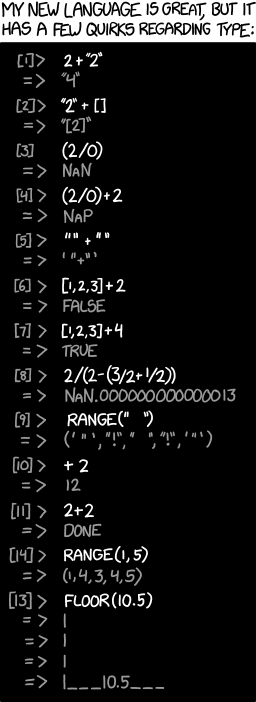
\includegraphics[scale=0.6]{types.png}\\
    \verb|https://xkcd.com/1537/|
\end{center}

\vspace{1cm}
\section*{Introduction}
Presque tous les langages de programmation relativement récents possèdent le typage comme fonctionnalité essentielle. Cela peut être une des raisons pour laquelle on choisirait un langage plutôt qu'un autre.

En effet, un programme bien typé empêche toute sorte d'opération incohérente entre plusieurs valeurs. Si le langage en question applique le typage au programme \textit{avant} la compilation (on dit qu'il est << statiquement typé >>), alors ces erreurs sont détectées avant l'exécution, ce qui permet d'éviter de nombreux problèmes...

Cependant, le typage ne permet pas seulement d'empêcher les erreurs : il permet par exemple de rendre un langage plus expressif et plus permissif, par exemple grâce au \textit{polymorphisme}. En connaissant le type d'une fonction, il est aussi plus facile de deviner ce qu'elle fait. Le typage sert donc comme outil de documentation.

Mais ces bénéfices ont un prix : il faut connaître le type de toutes les valeurs que l'on manipule avant l'exécution du programme. Dans certains langages de programmation possédant un système de types assez simple (comme le C), ce n'est pas vraiment un problème. Dans d'autres langages comme OCaml, qui donne accès au polymorphisme et donc à des combinaisons infinies de types, on serait bien embêté d'indiquer tous les types des étapes intermédiaires. On est même parfois obligé de le faire au risque que le compilateur/l'analyseur sémantique n'ait pas assez d'informations (voir les fichiers d'en-tête pour les modules en OCaml).

Au vu de ce problème, il existe des algorithmes permettant de retrouver les types des valeurs d'un programme sans que le programmeur n'ait à les écrire : on parle d'un algorithme \textbf{d'inférence de type}.

Dans cet exposé, on se propose de redécouvrir un algorithme d'inférence de type pour un système de type qui ressemble à celui d'OCaml : l'algorithme J. Pour cela, on étudiera d'abord un langage ultra-simplifié, le $\lambda$-calcul, auquel on ajoutera des types. On donnera ensuite des éléments de preuve pour montrer qu'un programme bien typé sera correctement évalué. Enfin, nous pourrons en déduire un algorithme d'inférence qui tente d'appliquer les règles de typage.


\section{Le lambda-calcul}

Pourquoi étudier un autre langage plutôt que celui d'OCaml ? Nous aurons par la suite besoin d'une manière de parler de l'évaluation d'un programme, et pour cela, le langage OCaml est trop gros. Une fois que l'on aura prouvé nos propriété sur les programmes bien typés, il sera en théorie très simple d'étendre les preuves sur toutes les constructions du langage OCaml.

Mais pour le moment, on décide de se réduire à un langage simpliste qui permet néanmoins toutes les opérations que peut exécuter OCaml. D'où l'intérêt de choisir un langage Turing-complet.

Un langage qui fonctionne parfaitement pour cette étude est le \textbf{lambda-calcul} (aussi noté $\lambda$-calcul), introduit dans les années 1930 par Alonzo Church. Dans les années 1940, il introduit une nouvelle version avec le typage : c'est le \textbf{lambda-calcul simplement typé}, aussi noté $\lambda^{\rightarrow}$

\subsection{Initiation au lambda-calcul et définitions}

Le lambda-calcul est un mini-langage dont les seules primitives sont les fonctions et les variables. On définit une manière d'écrire les fonctions, les variables et les applications de fonctions dans ce langage de manière condensée.

\begin{definition}
    On définit $\Lambda$, le langage des $\lambda$-termes à l'aide d'une grammaire non-contextuelle. 

    On prendra comme non-terminaux : $\mathcal{V}=\left\{E, X\right\}$. Notre alphabet sera constitué de deux symboles uniques '$\lambda$' et '$.$' réservés pour la syntaxe, auquel on ajoute tous les noms de variables que l'on souhaite.

    $$\Sigma = \left\{\lambda, .\right\}\cup\left\{a, b, \dots, x, y, \dots\right\}$$

    On désigne par $E$ le symbole initial, et les règles de production sont alors :

    \begin{equation*}
    \begin{aligned}
        E &\rightarrow X &\text{(variable)}\\
          &\rightarrow \lambda X.~ E &\text{(abstraction)}\\
          &\rightarrow E~E&\text{(application)}\\
        X &\rightarrow a~|~b~|~\dots~|~x~|~y~|~\dots
    \end{aligned}
    \end{equation*}
\end{definition}

\begin{remark}
    Une syntaxe plus concise pour la définition du langage des $\lambda$-termes est :

    \begin{equation*}
    \begin{aligned}
        e &:= x ~|~\lambda x.~e~|~e~e
    \end{aligned}
    \end{equation*}

    Au passage, ceci définit bien l'ensemble des $\lambda$-termes comme un ensemble inductif.
\end{remark}

Les $\lambda$-termes sont seules expressions autorisée dans le langage. Mais à quoi correspondent-elles ? Comme l'indiquent les annotations à côté de chaque règle de dérivation, un $\lambda$-terme décrit soit une variable $x$, soit une application d'une fonction $f$ à un autre terme $e$, soit une fonction elle-même, que l'on note $\lambda x.~e$ (où $x$ est l'argument).

Ainsi, lorsque l'on voit $\lambda x.~e$, on peut le lire << \textit{la fonction qui à $x$ associe $e$} >>.

En pratique, voilà ce que cela donne pour quelques fonctions usuelles.

\begin{example}
Prenons la fonction identité $x \mapsto x$. Le $\lambda$-terme correspondant serait :
$$\lambda x.~x$$

Et ensuite, si on voulait l'appliquer à $y$, on écrirait :
$$(\lambda x.~x)~y$$ 
\end{example}

\begin{example}
Un autre exemple, partons cette fois-ci d'une fonction en OCaml.

$$\verb|let f x y = x|$$

En OCaml, les fonctions ne prennent qu'un seul argument, mais on peut "émuler" la fonctionnalité de plusieurs arguments avec la curryfication :

$$\verb|let f = fun x -> fun y -> x|$$

Le $\lambda$-terme équivalent est alors :
$$\lambda x.~\lambda y.~x$$
\end{example}

Que ce cache-t-il derrière les variables $x$, $y$, etc ? Rien, ce sont des lambda-termes également, et deviendront soit des applications soit des fonctions lorsqu'on les évaluera.

\begin{definition}
    On notera dans toute la suite la fonction identité avec :
    $$\operatorname{id} = \lambda x.~x$$
\end{definition}

\subsection{$\alpha$-équivalence}

Si vous vous souvenez bien de votre cours sur la logique du premier ordre, les variables pouvaient être liées par un quantificateur $\forall$ ou $\exists$, et on disait qu'une telle variable était \textit{liée}, ou sinon, on disait qu'elle était \textit{libre}.

$$\exists \textcolor{red}{x} ~\mid~ \forall \textcolor{blue}{y}, ~\left(R(\textcolor{red}{x}) \implies R(\textcolor{blue}{y})\right)$$

Il en va de même pour les $\lambda$-termes.
\begin{definition}
    On dit qu'une variable $x$ d'un $\lambda$-terme est \textit{liée} si elle fait partie d'un terme de la forme ($\lambda x.$ \dots) :

    $$(\lambda a. ~\dots~(\lambda \textcolor{red}{x}.~ \dots ~ \textcolor{red}{x} ~ \dots))~\dots$$

    On dit que le $\lambda x.$ le plus proche de $x$ est son \textit{lieur}.

    Une variable est \textit{libre} dans un terme si elle n'y est pas liée.

    Enfin, pour $e\in\Lambda$, on peut noter $\operatorname{BV}(e)$ l'ensemble des liées dans $e$, et $\operatorname{FV}(e)$ l'ensemble des variables libres dans $e$.
\end{definition}

Qui dit << variable libre>> dit renommage : on peut renommer les variables dans un $\lambda$-terme sans que ce dernier ne << change de sens>>. Par contre, si l'on essaie de renommer une variable qui est déjà liée dans un terme, on obtient quelque chose de différence. Pour le voir avec des fonctions, j'ai le droit de faire ça :

$$(x\mapsto f(x))~~=~~(y\mapsto f(y))$$

mais pas ça, puisque je ne sais plus quelle variable est qui :
$$(x\mapsto f(x))~~\ne~~(f\mapsto f(f))$$

\begin{definition}
    On dit que deux $\lambda$-termes $e_1$ et $e_2$ sont \textit{$\alpha$-équivalents} s'ils sont égaux à renommage près. J'emploierai la notation suivante :
    
    $$e_1 \equiv_\alpha e_2$$
    
    On peut dire que l'on travaille \textit{module $\alpha$-équivalence}, car le nom des variables n'est pas important lorsque l'on effectue une opération sur les lambda-termes (on peut toujours renommer en un terme convenable).
\end{definition}

\begin{theorem}
    La relation d'$\alpha$-équivalence est une relation d'équivalence.

    \begin{preuve}
    Une relation d'équivalence est réfléxive, symétrique et transitive :
    \begin{itemize}
        \item Réflexivité : oui, en ne faisant aucun renommage.
        \item Symétrie : en appliquant les renommages inverses.
        \item Transitivité : si $e_1 \equiv_\alpha e_2,~e_2 \equiv_\alpha e_3$, on renomme $e_1$ en $e_2$ par les premiers renommages, puis $e_2$ en $e_3$ par les deuxièmes renommages, et donc $e_1 \equiv_\alpha e_3$
    \end{itemize}
    \end{preuve}
\end{theorem}

\begin{theorem}
    La relation d'$\alpha$-équivalence est une relation dite << de congruence >>, c'est-à-dire, si $e_1 \equiv_\alpha e_2$, alors
    \begin{itemize}
        \item $\lambda x.~e_1 \equiv_\alpha \lambda x.~e_2$
        \item $\forall e\in\Lambda, ~ e~e_1 \equiv_\alpha e~ e_2$
        \item $\forall e\in\Lambda, ~ e_1~e \equiv_\alpha e_2~e$
    \end{itemize}

    \begin{preuve}
    Pas besoin de détailler, il suffit juste de renommer la partie du $\lambda$-terme qui est importante.
    \end{preuve}
\end{theorem}

\subsection{Substitution}

Une opération similaire à l'$\alpha$ renommage est celle de substitution, consiste à renommer des variables non pas en autre variables, mais en d'autres $\lambda$-termes. C'est exactement ce que l'on fait avec des formules logiques.

Si j'ai une suite $\left(a_n\right)$ qui converge vers $l$, alors
$$\forall\epsilon>0, \exists n_0\in\mathbb{N}~\mid~\forall n\ge n_0, \left|a_n-l\right|<\epsilon$$

donc en prenant une limite $l=0$  (et une suite qui converge bien vers $0$) :

$$\forall\epsilon>0, \exists n_0\in\mathbb{N}~\mid~\forall n\ge n_0, \left|a_n-0\right|<\epsilon$$

On peut dire qu'on a réécrit la formule avec la substitution $\left[l\leftarrow0\right]$. Par contre, il faut faire attention : si j'avais appelé ma limite $n_0$, j'aurais obtenu une formule qui n'a plus de sens, car $n_0$ \underline{est lié dans la formule}.

Le principe est le même avec les $\lambda$-termes : on va remplacer des variables avec de nouveaux termes, à condition de ne pas transformer des variables liés en variables libres, ou vice-versa.

\begin{definition}
    Soit $x$ une variable et $a, b\in\Lambda$ deux lambda-termes. On définit par induction la substitution par $b$ de $x$ dans le terme $a$, que l'on note
    $$a\left[x\leftarrow b\right]$$
    par
    \begin{equation*}
    \begin{aligned}
        x[x \leftarrow b] = b&\hspace{1cm}\text{on remplace $x$ par $b$}\\
        y[x \leftarrow b] = y &\hspace{1cm}\text{\underline{si $x\ne y$}, pour ne pas remplacer la mauvaise variable}\\
        \left(a_1~a_2\right)[x \leftarrow b] = a_1[x \leftarrow b]~a_2[x \leftarrow b]&\hspace{1cm}\text{on remplace dans les deux termes de l'application}\\
        \left(\lambda x.~a_1\right)[x \leftarrow b] = \lambda x.~a_1&\hspace{1cm}\text{on ne peut pas substituer une variable déjà liée}\\
        \left(\lambda y.~a_1\right)[x \leftarrow b] = \lambda y.~\left(a_1[x \leftarrow b]\right)&\hspace{1cm}\text{\underline{si $y=x$ et $y\notin \operatorname*{FV}(b)$}, pour ne pas lier des $y$ venant de $b$}\\
    \end{aligned}
    \end{equation*}

    Lorsqu'une condition pour une substitution n'est pas remplie, on peut d'effectuer un $\alpha$-renommage pour éviter d'avoir des variables en commun.
\end{definition}

\begin{remark}
    On peut lire la notation $$a\left[x\leftarrow b\right]$$
    << la substitution de $x$ par $x$ dans $a$ >>, ou << $a$, en remplaçant toutes les occurences libres de $x$ par $b$ >>, etc.

    Par ailleurs, on retrouve aussi les notations équivalentes dans la littérature :

    $$a^{\left\{x\leftarrow b\right\}}$$
    $$a\left[b/x\right]$$
\end{remark}

\begin{example}
    $$\left(x~y\right)\left[y \leftarrow \lambda z.~ x\right] = x \left(\lambda z.~ x\right)$$
\end{example}

\begin{example}
    Dans cet exemple, on applique la substitution de manière incorrecte.
    \begin{equation*}
    \begin{aligned}
        \underbrace{\left(\lambda x.~x~y\right)}_{\text{$x$ lié}}\underbrace{\left[y\leftarrow \lambda z.~ x\right]}_{\text{$x$ libre}} &= \underbrace{\lambda x.~\left(x\left[y\leftarrow \lambda z.~ x\right]\right) \left(y\left[y\leftarrow \lambda z.~ x\right]\right)}_{\substack{\text{le $x$ qui était précédemment libre}\\\text{est désormais un argument (lié)}\\\text{???}}}\\
    \end{aligned}
    \end{equation*}

    Pour pouvoir l'effectuer correctement, on réécrit le $\lambda$-terme d'origine en renommant la variable $x$ liée (en $t$).
    $$\lambda x.~ x ~ y\equiv_\alpha\lambda t.~ t ~ y$$

    et donc

    \begin{equation*}
    \begin{aligned}
        \left(\lambda t.~ t ~ y\right)\left[y\leftarrow \lambda z.~ x\right]&=\lambda t. ~\left(t\left[y\leftarrow \lambda z.~ x\right]\right) \left(y\left[y\leftarrow \lambda z.~ x\right]\right)\\
        &=\lambda t. ~t~\left(\lambda z.~ x\right)~~~~~~~~~\text{ok}\\
    \end{aligned}
    \end{equation*}
\end{example}

Très vite, on va se rendre compte que cette opération va nous permettre enfin de manipuler les lambda-termes en tant que fonctions. En effet, lorsque l'on applique une fonction $f$ à une valeur $y$, on remplace les occurences libres et $x$ par $y$, et on enlève le << $f(x) =$ >>. Donc, pour un $\lambda$-terme, pour effectuer une application, on enlève le << $\lambda x.$ >>, puis on remplace $x$ par sa nouvelle valeur dans le reste.

\newpage
\subsection{Exécution par $\beta$-réduction}

Dès que l'on a un lambda-terme qui est l'application d'un terme $b$ à une lambda abstraction $\lambda x.~a$, on peut "évaluer" ce terme en calculant l'application : on remplace $x$ par $b$ dans $a$ (avec une substitution). Et ensuite, il n'y a plus qu'à répéter l'opération sur les nouveaux termes qui apparaissent. Ainsi, par exemple, le lambda-terme
$$\left(\lambda x.~f x\right) y$$
deviendrait
$$f~y$$

Définissons un opérateur qui met en relation deux $\lambda$-termes par ce procédé : c'est la $\beta$-réduction.

\begin{definition}
D'abord, on appelle un $\beta$-rédex un $\lambda$-terme de la forme: 
$$\left(\lambda x.~a\right) b$$
...où $a, b\in\Lambda$, et $x$ est une variable.

On note $\longrightarrow$ la relation de $\beta$-réduction, et on commence à mettre en relation tous les $\beta$-rédex avec un nouveau terme associé :
$$\underline{\left(\lambda x.~a\right) b} \longrightarrow a\left[x\leftarrow b\right]$$

Puis pour chaque $\lambda$-terme contenant au moins un rédex, on le met en relation avec lui-même, où on a remplacé le rédex par son terme associé selon la définition ci-dessus.

$$\left(\lambda t.~\dots~\left(\underline{\left(\lambda x.~a\right) b}\right)~\dots \right) \longrightarrow \left(\lambda t.~\dots~\left(a\left[x\leftarrow b\right]\right)~\dots \right)$$

Ceci constitue en son intégralité la relation de $\beta$-réduction. On notera également sa clôture refléxive et transitive $\longrightarrow^*$
\end{definition}

\begin{remark}
    Lorsque l'on effectue une étape de $\beta$-réduction, on peut souligner le rédex que l'on réduit pour le mettre en évidence.
\end{remark}

\begin{example}
    \begin{equation*}
    \begin{aligned}
    \operatorname{id} y &= \underline{\left(\lambda x.~x\right) y}\\
    &\longrightarrow x\left[x\leftarrow y\right]\\
    &=y
    \end{aligned}
    \end{equation*}
    
    \begin{equation*}
    \begin{aligned}
    \operatorname{id} \operatorname{id} &= \underline{\left(\lambda x.~x\right)~\left(\lambda x.~x\right)}\\
    &\longrightarrow \left(\lambda x.~x\right) = \operatorname{id}
    \end{aligned}
    \end{equation*}
\end{example}

\begin{example}
    \begin{equation*}
    \begin{aligned}
    \underline{\left(\lambda x.~\lambda y.~\lambda z.~y\right)~a}~b~c&\longrightarrow\underline{\left(\lambda y.~\lambda z.~y\right)~b}~c\\
    &\longrightarrow\underline{\left(\lambda z.~b\right)~c}\\
    &\longrightarrow b\\
    \end{aligned}
    \end{equation*}
\end{example}

On note dans toute la suite
$$\operatorname{app} = \lambda f.~\lambda x.~f~x$$
C'est le lambda-terme qui accepte un terme $f$, puis un argument $x$, et qui renvoie le terme $f~x$. C'est donc la fonction qui prend une fonction $f$, et qui l'applique à une argument $x$ voulu.

\begin{example}
    \begin{equation*}
    \begin{aligned}
        \operatorname{app} \operatorname{id} a&=\underline{\left(\lambda f.~\lambda x.~f~x\right)~\left(\lambda t.~t\right)}~a\\
        &\longrightarrow \underline{\left(\lambda x.~\left(\lambda t.~t\right)~x\right) a}\\
        &\longrightarrow \underline{\left(\lambda t.~t\right)~a}\\
        &\longrightarrow a
    \end{aligned}
    \end{equation*}

    On aurait pu le faire d'une autre manière :
    \begin{equation*}
    \begin{aligned}
        \operatorname{app} \operatorname{id} a&=\underline{\left(\lambda f.~\lambda x.~f~x\right)~\left(\lambda t.~t\right)}~a\\
        &\longrightarrow (\lambda x.~\underline{\left(\lambda t.~t\right)~x}) a\\
        &\longrightarrow \underline{\left(\lambda x.~x\right)~a}\\
        &\longrightarrow a
    \end{aligned}
    \end{equation*}
\end{example}

Voici un exemple où l'on peut réduire une infinité de fois :
\begin{example}
    Notons $\Delta = \lambda x.~x~x$ et calculons le terme suivant :
    \begin{equation*}
    \begin{aligned}
        \Delta~\Delta &= \underline{\left(\lambda x.~x~x\right) \left(\lambda x.~x~x\right)}\\
        &\longrightarrow \left(x\left[x\leftarrow \left(\lambda x.~x~x\right)\right]\right) \left(x\left[x\leftarrow \left(\lambda x.~x~x\right)\right]\right)\\
        &= \left(\lambda x.~x~x\right) \left(\lambda x.~x~x\right)\\
        &=\Delta~\Delta
    \end{aligned}
    \end{equation*}

    Donc $\Delta~\Delta \longrightarrow^* \Delta~\Delta$. On dit que ce $\lambda$-terme diverge.
\end{example}

Enfin, pour pouvoir exprimer que deux $\lambda$-termes sont << égaux >> dans le sens où ils se comportent de la même manière, on peut définir une relation d'équivalence sur $\Lambda$ avec la $\beta$-réduction.

\begin{definition}
    On désigne par $\equiv_\beta$ la clôture réflexive, transitive et symétrique de la $\beta$-réduction. C'est-à-dire que c'est la plus petite relation telle que :
    \begin{itemize}
        \item $\forall (e, e') \in\Lambda^2,~e\longrightarrow e' \implies~e\equiv_\beta e'$
        \item Réflexivité : $\forall e \in\Lambda,~e \equiv_\beta e$
        \item Symétrie : $\forall (e, e') \in\Lambda^2,~e\equiv_\beta e' \iff e' \equiv_\beta e$
        \item Transitivité : $\forall (a, b, c) \in\Lambda^3,~a\equiv_\beta b~\text{et}~b\equiv_\beta c \implies a \equiv_\beta c$
    \end{itemize}
\end{definition}

Autrement dit, intuitivement, deux lambda-termes sont $\beta$-équivalents (<< égaux >>) ils peuvent s'évaluer à un même lambda-terme. C'est un peu la même chose que pour les calculs mathématiques : deux expressions mathématiques sont égales si je peux appliquer des règles de calcul des deux côtés pour arriver au même résultat :
$$\underbrace{(1 + 1) = 2}_{\substack{\text{par addition}\\\text{sur les entiers}}}~~~~~~\text{et}~~~~~~\underbrace{(3-1)=2}_{\substack{\text{par soustraction}\\\text{sur les entiers}}}~~~~~~\text{donc}~~~~~~\text{<< }1+1=3-1\text{ >>}$$

\begin{theorem}
    Conséquence : si $a \longrightarrow^* c$ et $b \longrightarrow^*c$, alors $a \equiv_\beta c$.
    \begin{preuve}
        $a = a_1 \longrightarrow a_2 \longrightarrow \dots \longrightarrow c$, donc $a = a_1 \equiv_\beta a_2 \equiv_\beta \dots \equiv_\beta c$, d'où $a \equiv_\beta c$ par transitivité, et pareil pour $b \equiv_\beta c$. Encore par transitivité, on a $a \equiv_\beta b$.
    \end{preuve}
\end{theorem}

La relation $\equiv_\beta$ est clairement une relation d'équivalence étant donné sa définition.

\subsection{Stratégie de réduction}

Les quelques derniers exemples montrent qu'il y a plusieurs façons d'évaluer le même $\lambda$-terme par $\beta$-réduction, et que, parfois, on peut ne jamais s'arrêter.
On peut alors mettre en place plusieurs stratégies qui dictent les rédex qu'on a le droit de réduire ou pas. 

\begin{definition}
    Un $\lambda$-terme est dit sous forme \textit{normale}, si, pour une stratégie de réduction donnée, il n'existe aucun autre terme obtenu par $\beta$-réduction.
\end{definition}

La stratégie dite << \textit{appel par nom} >>, aussi notée {\scshape{call-by-name}}, impose que l'on évalue toujours les rédex les plus à gauche, les plus extérieurs. Cette stratégie a pour conséquence que l'on évalue substitue toujours un argument par son terme associé lorsque l'on évalue une fonction. Cette stratégie a le mérite de toujours atteindre sa forme normale lorsqu'elle existe.

Une autre stratégie, appelée << \textit{appel par valeur} >>, notée {\scshape{call-by-value}}, impose, elle, que l'on réduise les arguments d'une fonction \underline{avant} de les appliquer. Cette stratégie est celle employée par la plupart des langages de programmation, y compris C et OCaml.

\begin{example}
    Le $\lambda$-terme suivant est sous forme normale selon la stratégie {\scshape{call-by-value}}, car on ne peut pas évaluer l'intérieur de la fonction sans d'abord l'appliquer à tous les arguments.
    $$(\lambda y.~(\lambda x.~f~x)~y)$$
    Même s'il y a un rédex, $(\lambda x.~f~x)~y$, dans la $\lambda$-abstraction, la stratégie interdit sa réduction, et donc il n'y a rien à faire.
\end{example}

\section{Programmer avec le lambda-calcul}
On a vu comment utiliser le $\lambda$-calcul comme outil permettant de modéliser le calcul d'applications de fonctions à d'autre fonctions et d'autres variables. Mais si les fonctions sont les seules primitives du langage, est-il vraiment utile ? Que peut-on faire d'autre comme calcul qui ressemble plus à ceux d'un vrai langage de programmation ?

\subsection{Booléens de Church}
Dans le $\lambda$-calcul, on n'a que les fonctions et les variables comme valeurs, mais en OCaml, les booléens sont deux constantes, \verb|true| et \verb|false|, qui constituent le type \verb|bool|. Pour pouvoir faire l'analogie, il faudrait définir un $\lambda$-terme qui correspond à \verb|true|, et un autre qui correspond à \verb|false|.

Nous allons voir deux lambda-termes qui remplissent parfaitement ce devoir. Ils ont été utilisés pour la première fois par Alonzo Church.

\begin{definition}
    \begin{equation*}
    \begin{aligned}
        \operatorname{true} &= \lambda x.~\lambda y.~x\\
        \operatorname{false} &= \lambda x.~\lambda y.~y\\
    \end{aligned}
    \end{equation*}
\end{definition}

Ainsi, le booléen \verb|true| est représenté par la fonction qui prend deux arguments, $x$ et $y$, et qui renvoie juste le premier, $x$. Similairement, le booléen \verb|false| est représenté par la fonction qui prend deux arguments $x$ et $y$, mais qui ne renvoie que le deuxième, $y$.

Pour comprendre cette représentation, considérons le fonctionnement des booléens en OCaml. Que peut-on faire avec des booléens ? Ce sont des valeurs simples, que l'on peut stocker et manipuler, ou même combiner avec des portes logiques ou autres formules. Mais principalement, les booléens servent à effectuer des tests dans un programme. Comme dans, par exemple :

\begin{equation*}
    \texttt{if condition then x else y}
\end{equation*}

\newpage
Lorsque cette expression est évaluée, il y a deux cas possibles :
\begin{itemize}
    \item \verb|condition = true| : alors on a \texttt{if true then }\underline{\texttt{x}}\texttt{ else y}, qui donne simplement \verb|x|.
    \item \verb|condition = false| : similairement, on a \texttt{if false then x else }\underline{\texttt{y}}, soit juste \verb|y|.
\end{itemize}

En quelques sortes, la structure de contrôle \verb|if-then-else| en OCaml agit comme si l'on avait appliqué \verb|x| et \verb|y| a une fonction qui choisit soit \verb|x| soit \verb|y| : et cette fonction n'est autre que \verb|true|, ou \verb|false| telles que nous les avons définies. Si bien que l'on peut redéfinir cette structure de contrôle :
$$\operatorname{if} = \lambda b.~\lambda x.~\lambda y.~b~x~y$$

Ici, ce $\lambda$-terme prend un lambda-terme $b$ en argument, et l'applique à deux autres arguments $x$ et $y$. Justement, si $b$ se trouve être true, alors on a
\begin{equation*}
\begin{aligned}
    \operatorname{if}~\operatorname{true}~a~b&=\underline{\underline{\underline{(\lambda b.~\lambda x.~\lambda y.~b~x~y)~\operatorname{true}}~a}~b}\\
    &\longrightarrow^*\operatorname{true}~a~b\\
    &=\underline{(\lambda x.~\lambda y.~x)~a}~b\\
    &\longrightarrow \underline{(\lambda y.~a)~b}\\
    &\longrightarrow a\\
\end{aligned}
\end{equation*}

Ce qui est bien le résultat que l'on cherchait à obtenir !
Similairement :
\begin{equation*}
\begin{aligned}
    \operatorname{if}~\operatorname{false}~t~f&\longrightarrow^*\operatorname{false}~t~f\\
    &=(\lambda x.~\lambda y.~y)~t~f\\
    &\longrightarrow^* f
\end{aligned}
\end{equation*}

On peut alors commencer à construire des lambda-termes qui commencent à ressembler à des expressions d'un langage de programmation, et même définir des opération que l'on connaît déjà :
\begin{definition}
    Opération sur les booléens :
    \begin{equation*}
    \begin{aligned}
        \operatorname{not} &= \lambda b.~\operatorname{if}~b~\operatorname{false}~\operatorname{true}\\
        \operatorname{and} &= \lambda a. ~\lambda b.~ \operatorname{if}~a~b~\operatorname{false}\\
        \operatorname{or} &= \lambda a. ~\lambda b.~ \operatorname{if}~a~\operatorname{true}~b\\
        \operatorname{xor} &= \lambda a. ~\lambda b.~ \operatorname{or} \left(\operatorname{and}~a~\left(\operatorname{not}~b\right)\right) ~ \left(\operatorname{and}~b~\left(\operatorname{not}~a\right)\right)\\
    \end{aligned}
    \end{equation*}
\end{definition}

\begin{example}
    \begin{equation*}
    \begin{aligned}
        \operatorname{if}~\left(\underline{\operatorname{and}~\operatorname{true}~\operatorname{false}}\right)~x~\left(\operatorname{if}~\left(\operatorname{or}~\operatorname{false}~\operatorname{true}\right)~y~z\right)&\longrightarrow^*\operatorname{if}~\operatorname{false}~x~\left(\operatorname{if}~\left(\operatorname{or}~\operatorname{false}~\operatorname{true}\right)~y~z\right)\\
        &\longrightarrow^*\operatorname{if}~\left(\underline{\operatorname{or}~\operatorname{false}~\operatorname{true}}\right)~y~z\\
        &\longrightarrow^*\operatorname{if}~\operatorname{true}~y~z\\
        &\longrightarrow^*\operatorname{true}~y~z\\
        &\longrightarrow^*y
    \end{aligned}
    \end{equation*}
\end{example}

\begin{remark}
    On peut remarquer qu'à chaque fois que l'on écrit << if >>, il est redondant puisqu'il disparait éventuellement. En effet, et la raison pour cela est que
    $$\operatorname{if}~b~x~y \equiv_\beta b~x~y$$
    car
    \begin{equation*}
    \begin{aligned}
        \underline{\left(\lambda b.~\lambda x.~\lambda y.~b~x~y\right)~b'}~x'~y'\longrightarrow\underline{\left(\lambda x.~\lambda y.~b'~x~y\right)~x'}~y'&\longrightarrow\underline{\left(\lambda y.~b'~x'~y\right)~y'}\\&\longrightarrow b'~x'~y'\\
    \end{aligned}
    \end{equation*}
\end{remark}

\subsection{Entiers naturels de Church}

Comme avec les booléens, on a vu que l'on pouvait se servir de lambda-termes pour représenter les valeurs << vrai >> ou << faux >>. Observons que pour cela, on a utilisé les variables liées dans une $\lambda$ abstraction pour << stocker des informations >> :
$$\operatorname{true} = \underbrace{\lambda x.~~~~~\lambda y.~~~~}_{\substack{\text{valeurs stockées}\\\text{dans ces variables}}}~x$$

Plus précisément, un << booléen >> de Church stocke la valeur à renvoyer s'il est vrai (dans $x$), et stocke la valeur à renvoyer s'il est faux (dans $y$).

Ainsi, si on arrive à utiliser dans lambda-termes que l'on stocke dans une abstraction, qui permettent de calculer un entier, alors on pourra utiliser des lambda-termes comme des entiers ! Mais d'abord, qu'est-ce qu'un entier ?

\begin{definition}
    Définissons les entiers naturels $\mathbb{N}$ de la manière suivante comme un ensemble inductif :
    $$n := 0~\mid~S(n)$$
    où $0$ est un constructeur d'arité 0, et $S$ est un constructeur d'arité 1.
\end{definition}

Donc selon cette définition, on a $3=S(S(S(0)))$, ou bien $N=\underbrace{S(S(\dots(S}_\text{$N$ fois}(0))))$

On peut alors le voir sous un autre angle. Pour construire un entier $N$, on se donne une fonction << successeur >> $S$, et on l'applique $N$ fois à un élément initial << 0 >>, très exactement comme une suite récurrente définie par une fonction, de terme initial 0. Ceci est avantageux car le $\lambda$-calcul modélise parfaitement le calcul d'applications de fonctions. On va alors créer un $\lambda$-terme qui, étant donné deux arguments $S$ et $z$ (zéro), appliquera $S$ un certain nombre de fois à $z$ pour \textit{représenter} un entier naturel :

Commençons simplement, pour calculer zéro, j'applique zéro fois la fonction successeur à zéro lui-même.
$$0=\lambda S.~\lambda z.~z$$
Notons que la définition de 0 comme $\lambda$-terme est bien une fonction, et pas juste $z$ : sinon, je ne pourrais rien faire avec $z$, ni $S$ ! (ce sont juste des variables).
Je poursuis avec l'entier suivant, il faut appliquer une fois la fonction successeur à zéro :
$$1=\lambda S.~\lambda z.~S~z$$
Puis deux, trois, \dots, $N$ fois :
\begin{definition}
    \begin{equation*}
    \begin{aligned}
        0 &= \lambda S.~\lambda z.~z\\
        1 &= \lambda S.~\lambda z.~S~z\\
        2 &= \lambda S.~\lambda z.~S~(S~z)\\
        3 &= \lambda S.~\lambda z.~S~(S~(S~z))\\
        &\vdots\\
        \boxed{N}&=\lambda S.~\lambda z.~\underbrace{S~(S~(\dots~S~(S}_\text{$N$ fois}~z)))~~~~~~~~~~~~\substack{\text{où $\boxed{N}$ désigne l'écriture décimale de $N$}\\\text{et non le caractère litéral << N >>}}
    \end{aligned}
    \end{equation*}
    Ces $\lambda$-termes sont la représentation des entiers naturels de Church, aussi appelés les << entiers de Church >>.
\end{definition}

Remarquons tout de suite quelque chose : \underline{tous mes entiers sont toujours de la forme $\lambda S.~\lambda z.~ (\dots)$} où $S$ est appliqué un nombre fini de fois à $z$ dans les parenthèses. Ceci est important, et nous aidera à savoir si nous sommes en train d'écrire un entier ou non. Si nous voulons créer un entier de Church, il faudra s'assurer que le lambda terme que l'on écrit est bien de cette même forme.

\newpage
Tentons ainsi de définir les opérations usuelles sur les entiers naturels avec cette nouvelle définition.

\subsubsection{Successeur}

Que faut-il faire pour incrémenter un entier ? Par définition, il faut appliquer la fonction successeur $S$. Donc, si j'ai un lambda-terme $n=\lambda S.~\lambda z.~(\dots)$, qui appliquer $n$ fois $S$ à $z$, il faut que j'applique une dernière fois $S$ au résultat de l'appel $n~S~z$.

La fonction successeur sur les entiers de Church ressemble donc à ceci: 

$$\operatorname{succ} = \lambda n.~\lambda S.~\lambda z.~S \left(n~S~z\right)$$

Il peut parfois être difficile de comprendre ce que fait un lambda-terme juste en regardant son écriture. Détaillons plus spécialement la $\beta$-réduction d'un appel à $\operatorname{succ}$.
\begin{itemize}
    \item Le premier argument, ($\lambda n. (\dots) $) est l'entier de Church dont on prend le successeur : il faut donc se rappeler que c'est un lambda-terme de la forme $$\lambda S.~\lambda z.~ (\dots)$$ qui calcule $S^n(z)$.
    \item Il n'y a aucun autre argument à prendre, donc on doit maintenant retourner un entier de Church.
    $$\lambda n.~ \underbrace{\dots}_{\text{entier de Church}}$$
    Ainsi, le lambda-terme qui suit l'argument $n$ doit être de la forme $\lambda S.~\lambda z.~ (\dots)$, qui applique $n+1$ fois $S$ à la constante $z$. On commence donc par écrire les arguments $\lambda S$ et $\lambda z$ :
    $$\underbrace{\lambda n.}_\text{argument $n$}~\left(\underbrace{\lambda S.~\lambda z.}_\text{écriture d'un entier de Church}~\left(\underbrace{(\dots)}_\text{calcul de $S^{n+1}(z)$}\right)\right)$$

    \item Pour le calcul de $S^{n+1}(z)$, on peut s'appuyer sur le calcul qu'effectue $n$ lorsqu'on lui passe les arguments $S$ et $z$. Par définition, $n~S~z$ calcule $\underbrace{S(S(\dots S}_\text{$n$ fois}(z)))$. Il ne reste plus qu'à appliquer $S$ une dernière fois !
    $$S~(n~S~z)$$
    \dots ce qui donne bien $\underbrace{S(\underbrace{S(S(\dots S}_\text{$n$ fois}}_{\text{$n + 1$ fois}}(z))))$, c'est à dire, par définition, $\boxed{n+1}$ !
\end{itemize}

Pour résumer :
$$\operatorname{succ} = \underbrace{\lambda n.}_\text{argument $n$}~\left(\underbrace{\lambda S.~\lambda z.}_\text{écriture d'un entier de Church}~\left(
    \underbrace{S~\underbrace{(n~S~z)}_\text{calcul de $S^n(z)$}}_\text{calcul de $S^{n+1}(z)$}
\right)\right)$$

\begin{example}
    Pour comprendre la réduction d'un appel à $\operatorname{succ}$, regardons en détail cet exemple
    \begin{equation*}
    \begin{aligned}
        \operatorname{succ}~3 &= \underline{\left(\lambda n.~\lambda S.~\lambda z.~S \left(n~S~z\right)\right)~\left(\lambda S.~\lambda z.~ S(S(S~z))\right)}\\
        &\longrightarrow \lambda S.~\lambda z.~S \left(\underline{\underline{\left(\lambda S.~\lambda z.~ S(S(S~z))\right)~S}~z}\right)\\
        &\longrightarrow^* \lambda S.~\lambda z.~S\left(S(S(S~z\right)~~~~~~~~~~~~~~~~~~~~~\substack{\text{qui est bien sous la forme}\\\text{d'une entier de Church !}}\\
        &\equiv_\beta 4
    \end{aligned}
    \end{equation*}
\end{example}

\subsubsection{Addition}
Similairement, à la place de juste calculer le successeur une dernière fois sur un entier de Church, on peut utiliser deux entiers de Church $n$ et $m$ pour calculer les $n+m$ appels à $S$ sur zéro. En effet, pour visualiser cela, on peut utiliser une propriété usuelle sur les puissances de fonctions :
$$f^{a+b}(x)=f^a f^b (x)=f^a(f^b(x))$$
Donc, pour calculer l'entier $n + m$ à l'aide des successeurs :
$$\begin{cases}
    n = S^{n}(0)\\
    m = S^{m}(0)\\
\end{cases}\implies n + m = S^{n}(S^{m}(z))$$

D'après ce qui a été vu avec le $\lambda$-terme successeur, il est facile de construire le $\lambda$-terme qui performe l'addition de deux entiers de Chruch :
$$\operatorname{add} = \lambda n.~\lambda m.~\lambda S.~\lambda z. ~ n~S~(m~S~z)$$

Encore une fois, il est compliqué de comprendre ce que fait un terme juste en regardant son écriture, donc voici une écriture plus détaillée (je ne vais pas repasser sur la même explication pour la fonction successur) :
$$\operatorname{add} = \underbrace{\lambda n.~\lambda m.}_\text{argument $n$ et $m$ de l'addition}~\left(\underbrace{\lambda S.~\lambda z.}_\text{écriture d'un entier de Church}~\left(\underbrace{n~S~\left(\underbrace{m~S~z}_\text{calcul de $S^m(z)$}\right)}_\text{calcul de $S^{n+m}(z)$}\right)\right)$$

Une autre façon de le voir est que, dans le calcul $n~S~(m~S~z)$, le terme $m~S~z$ devient le << nouveau zéro >> pour le calcul de $S^n(\text{nouveau zéro})$, sauf que ce zéro est en fait l'entier $m$. Cela a pour effet d'appliquer $n$ fois $S$ à ce nouveau zéro, et par extension, $n + m$ fois $S$ au vrai zéro ($0$).

\begin{example}
    Pour le voir avec un exemple (addition de $2$ et $3$):
    \begin{equation*}
    \begin{aligned}
        \operatorname{add}~2~3&=\underline{\underline{\underbrace{\left(\lambda n.~\lambda m.~\lambda S.~\lambda z. ~ n~S~(m~S~z)\right)}_\text{add}~\underbrace{\left(\lambda S.~\lambda z.~ S(S~z)\right)}_2}~3}\\
        &\longrightarrow^* \lambda S.~\lambda z. ~ \underbrace{\left(\lambda S.~\lambda z.~ S(S~z)\right)}_2~S~(3~S~z)\\
        &\longrightarrow^* \lambda S.~\lambda z. ~ \underline{\underline{\underbrace{\left(\lambda S.~\lambda z.~ S(S~z)\right)}_2~S}~(3~S~z)}\\
        &\longrightarrow^*\lambda S.~\lambda z.~ S(S(3~S~z))\\
        &= \lambda S.~\lambda z.~ S(S(\underline{\underline{(\underbrace{\lambda S.~\lambda z.~S(S(S~z))}_3)~S}~z}))\\
        &\longrightarrow^* \lambda S.~\lambda z.~S(S(S(S(S~z))))\\
        &\equiv_\beta 5
    \end{aligned}
    \end{equation*}
    
    Donc << $2+3=5$ >>, \dots enfin, $\operatorname{add}~2~3\equiv_\beta 5$
\end{example}

Le $\lambda$-terme d'addition va nous permettre d'exprimer les autres opérations sur les entiers. Même la fonction successeur : en effet, le successeur d'un entier $n$ est $n + 1$.

\begin{theorem}
    Expression de $\operatorname{succ}$ à l'aide de $\operatorname{add}$ :
    $$\operatorname{succ}\equiv_\beta \operatorname{add}~1$$
    Autrement dit, la fonction successeur est parfaitement ($\beta$-)équivalente à la fonction qui ajoute 1.

    \begin{preuve}
        On vérifie par calcul que $\operatorname{add}~1$ est bien $\beta$-équivalent à $\operatorname{succ}$ :

        \begin{equation*}
        \begin{aligned}
            \operatorname{add}~1&=\underline{\left(\lambda n.~\lambda m.~\lambda S.~\lambda z.~n~S~(m~S~z)\right)~\left(\lambda S.~\lambda z.~ S~z\right)}\\
            &\longrightarrow \lambda m.~\lambda S.~\lambda z.~\underline{\underline{\left(\lambda S.~\lambda z.~ S~z\right)~S}~(m~S~z)}\\
            &\longrightarrow^* \lambda m.~\lambda S.~\lambda z.~S (m~S~z)\\
            &\equiv_\alpha \lambda n.~\lambda S.~\lambda z.~S (n~S~z)\\
            &= \operatorname{succ}
        \end{aligned}
        \end{equation*}
        D'où le résultat.
    \end{preuve}
\end{theorem}

\subsubsection{Multiplication}

De la même manière, on utilise les propriété de calcul sur les puissances des fonction pour se donner une idée de comment écrire un lambda-terme de multiplication sur les entiers naturels de Church.
$$f^{ab}(x)=\left(f^a\right)^b(x)=\underbrace{f^a(f^a(\dots f^a}_\text{$b$ fois}(x)))$$
On remarque que cette écriture ressemble beaucoup à $S^m(z)$, sauf que le << nouveau successeur >> devient $S^n$, qui n'est autre que la fonction qui ajoute $n$ à un entier. Cela paraît évident : la multiplication est en réalité la répétition d'une addition. En utilisant donc $\operatorname{add}$ défini précédemment, on peut définir $\operatorname{mul}$ :
$$\operatorname{mul} = \lambda n.~\lambda m.~m~(\operatorname{add}~n)~0$$

Comme toujours, voici une écriture détaillée, qui bizarrement, cette fois, a l'air plus simple :
$$\operatorname{mul} = \underbrace{\lambda n.~\lambda m.}_{\substack{\text{arguments $n$ et $m$} \\ \text{de la multiplication}}}~\left(\underbrace{m~\underbrace{(\operatorname{add}~n)}_{\substack{\text{nouveau successeur $S^n$}\\\text{qui fait $+n$}}}~0}_\text{calcul de $S^{m\times n}(z)$}\right)$$

Quelque chose a changé par rapport aux autres opérateurs usuels... il n'y a plus l'écriture d'un entier de Church ($\lambda S.~\lambda z.$) après les arguments $n$ et $m$. De même, à cause de cela, le zéro $z$ n'est plus dans l'écriture, et \underline{a été remplacé par le $\lambda$-terme 0}. Pourquoi ?

Pour comprendre cela, rappelons nous qu'un entier de Church est en réalité une fonction qui à $f$ et $x$ associe $f^{n}(x)$ (où $n$ est un certain entier naturel). Sous l'écriture mathématiques :
$$\boxed{n} = (f, x) \mapsto \underbrace{f(f(\dots f}_\text{$n$ fois}(x)))$$

Donc lorsque l'on écrit $m~(\operatorname{add} n)~0$, on calcul l'application de $\operatorname{add}n$, $m$ fois à zéro. Or, le $\lambda$-terme $\operatorname{add}n$ prend un argument un autre $\lambda$-terme sous la forme d'un entier de Church. Ici, on commence à partir de zéro, donc il faut l'appliquer à l'entier de Church nul 0, et non la constante $z$ !

\newpage
\begin{example}
    \begin{equation*}
    \begin{aligned}
        \operatorname{mul}4~5&\longrightarrow^* 4~(\operatorname{add}5)~0\\
        &= \underline{\underline{\left(\lambda S.~\lambda z.~ S(S(S(S~z)))\right)~(\operatorname{add}5)}~0}\\
        &\longrightarrow^* (\operatorname{add}5)((\operatorname{add}5)((\operatorname{add}5)(\underline{\operatorname{add}5~0})))\\
        &\equiv_\beta (\operatorname{add}5)((\operatorname{add}5)(\underline{\operatorname{add}5~5}))\\
        &\equiv_\beta (\operatorname{add}5)(\underline{\operatorname{add}5~10})\\
        &\equiv_\beta \underline{\operatorname{add}5~15}\\
        &\equiv_\beta 20
    \end{aligned}
    \end{equation*}

    Donc $\operatorname{mul}4~5 \equiv_\beta 20$, c'est-à-dire $4\times5=20$.
\end{example}

\subsubsection{Exponentiation}

Avec la construction du dernier opérateur, on peut généraliser la construction du lambda-terme pour l'opération qui répète une autre opération précédente déjà définie. En l'occurrence, l'exponentiation $a^b$ est la répétition $b$ fois de la multiplication par $a$, en partant du neutre 1.
$$\operatorname{exp}=\lambda n.~\lambda m.~m~(\operatorname{mul}n)~1$$

\begin{example}
    \begin{equation*}
    \begin{aligned}
        \operatorname{exp}2~3&\longrightarrow^* (\operatorname{mul} 2)((\operatorname{mul} 2) (\underline{\operatorname{mul} 2~1}))\\
        &\equiv_\beta (\operatorname{mul} 2)(\underline{\operatorname{mul} 2~2})\\
        &\equiv_\beta \underline{\operatorname{mul} 2~4}\\
        &\equiv_\beta 8
    \end{aligned}
    \end{equation*}

    Donc $\operatorname{exp}2~3\equiv_\beta 8$, c'est-à-dire $2^3=8$.
\end{example}

\begin{remark}
    On peut généraliser ce procédé pour n'importe quelle opération qui répète une opération précédemment définie. 
    
    Par exemple, la \textit{tétration} est la répétition de l'exponentiation, et se note $\,^b a$, ou encore $a \uparrow\uparrow b$. Donc, pour $2\uparrow\uparrow4$, on a $2^{2^{2^{2}}}=2^{2^4}=2^{16}=65~536$. Et le lambda-terme qui correspondant à la tétration est :
    $$\operatorname{tetra}=\lambda n.~\lambda m.~m~(\operatorname{exp} n)~1$$ 

    Puis ensuite, il y a la pentation, qui se note $a\uparrow\uparrow\uparrow b$. 
    
    Exemple : $2\uparrow\uparrow\uparrow4=2\uparrow\uparrow2\uparrow\uparrow2\uparrow\uparrow2=2\uparrow\uparrow2\uparrow\uparrow4=2\uparrow\uparrow 65~536=\underbrace{2^{2^{.^{.^{.^2}}}}}_\text{65536 fois}$ qui est astronomiquement grand. Ce qui se calcule par :
    $$\operatorname{penta}=\lambda n.~\lambda m.~m~(\operatorname{tetra} n)~1$$

    Enfin, on peut noter $\uparrow^p$ l'opérateur obtenu répétant cette construction $p$ fois. (Exemple : $\uparrow\uparrow\uparrow=\uparrow^3$)
    $$\forall p\in\mathbb{N},~~\uparrow^{p+1} = \lambda n.~\lambda m.~m~\left(\uparrow^p n\right)~1$$
\end{remark}

\subsection{Listes finies}
L'étude des entiers de Church nous a montré que les fonction itérées pouvait être bien utile pour effectuer des calculs. En particulier, à l'aide d'une fonction $S$ itérée un certain nombre de fois sur une constante $z$, on a pu construire tous les entiers naturels, ainsi qu'une infinité d'opérations sur ces derniers.

Avec ce nouveau pouvoir, on va construire quelque chose de plus général: les listes finies. Mais pour cela, il faut d'abord définir leur structure.

\begin{definition}
    Soit $A$ un ensemble. On définit l'ensemble des listes finies, noté $\operatorname{List}(A)$ comme un ensemble inductif :
    \begin{equation*}
    \begin{aligned}
        L &:= \operatorname{Empty}\\
        &\mid~\operatorname{Cons}(x, L)~~~~~~~~~\text{où $x\in A$}
    \end{aligned}
    \end{equation*}

    Empty est un constructeur constant (d'arité 0), et Cons est un constructeur d'arité 2, de la forme $A\times L \to L$.
\end{definition}

\begin{remark}
    Cette définition correspond à la définition des listes en OCaml.

    $$\texttt{type 'a list = }\underbrace{\texttt{[]}}_\text{Empty}\texttt{ | }\underbrace{\texttt{(::)}}_\text{Cons}\texttt{ of 'a * 'a list}$$
\end{remark}

\begin{example}
    La liste $\left[1, 2, 3\right]$ est représentée par Cons(1, Cons(2, Cons(3, Empty))).
\end{example}

Exactement comme pour les entiers naturels, on va se munir de deux lambda-termes correspondant à Empty et Cons, puis on va les utiliser pour calculer des listes à l'aide d'applications sur ces lambda-termes.

On appellera lambda-termes $C$ et $e$ Ainsi, les listes de $\operatorname{List}(A)$ seront des lambda-termes de la forme suivante $$\lambda C.~ \lambda e.~ C~a_1~(C~a_2~\dots~(C~a_n~e))~~~~~~~~~~~~~~\text{où $a_1, \dots, a_n$ sont les $n$ éléments de la liste}$$

Encore une fois, $C$ et $e$ sont des variables arbitraires qui sont des arguments dans des $\lambda$-abstractions, et non pas des constantes, car sinon on ne pourrait rien faire avec ! Il se s'agit pas de définir ce que font $C$ et $e$, mais plutôt de les utiliser pour décrire la forme d'une liste.

Dans toute la suite, je m'autorise à utiliser la notation $\left[a_1, \dots, a_n\right]$ pour désigner des listes représentées par un lambda-terme.

\begin{definition}
    \begin{equation*}
    \begin{aligned}
        \operatorname{empty} &= \lambda C.~\lambda e.~e &\substack{\text{qui correspond à la liste []}}\\
        \operatorname{cons} &= \lambda x.~\lambda L.~ \lambda C.~\lambda e.~C~x~(L~C~e) ~~~~~~~~ &\substack{\text{qui construit la liste Cons($x$, $L$)}\\\text{à partir de $x\in A$ et d'une liste $L$}}\\
    \end{aligned}
    \end{equation*}
\end{definition}

Le lambda-terme $\operatorname{empty}$ est simple à comprendre. C'est la représentation de la liste vide [] : étant donné le constructeur $C$ et le symbole vide $e$, il renvoie le symbole vide. On remarquera que ce lambda-terme est $\alpha$-équivalent à $0$ et à $\operatorname{false}$ : cela n'a rien à voir, mais il se trouve que le fonctionnement de ces objets est le même.

Cependant, comprendre $\operatorname{cons}$ est moins évident. Une écriture détaillée permet de mieux le voir :
$$\operatorname{cons} = \underbrace{\lambda x.~\lambda L.}_{\substack{\text{l'élément $x \in A$ à ajouter en tête}\\\text{et la liste $L$ qui deviendra la queue}}}~\left(\underbrace{\lambda C.~\lambda e.}_\text{écriture d'une liste}~\left(\underbrace{C~x~\underbrace{\left(L~C~e\right)}_\text{calcul de la liste $L$}}_\text{dernière construction avec $x$ en tête}\right)\right)$$

Ceci devrait paraître similaire à la construction des entiers de Church. Les listes commencent par $(\lambda C.~\lambda e.)$, toujours.

\begin{example}
    La liste [1, 2, 3] (où 1, 2 et 3 sont des entiers de Church) est représentée par
    $$\operatorname{cons}~1~(\operatorname{cons}~2~(\operatorname{cons}~3~\operatorname{empty}))$$
    qui est $\beta$-équivalente à
    $$\lambda C.~\lambda e.~C~1~(C~2~(C~3~e))$$
\end{example}

\subsubsection{Concaténation}

En une liste $L_2$ comme une liste << vide >> pour une autre liste $L_1$, on peut effectuer la concaténation $L_1L_2$ en calculant la liste $L_2$, puis en la passant comme constructeur vide pour le calcul de $L_1$.

$$\operatorname{concat} = \lambda L_1.~\lambda L_2.~\lambda C.~\lambda e.~ L_1~C~(L_2~C~e)$$

L'explication est la même que pour les entiers.
\begin{example}
\begin{equation*}
\begin{aligned}
    \operatorname{concat}~[1, 2, 3]~[4, 5, 6]&=\underline{\underline{\left(\lambda L_1.~\lambda L_2.~\lambda C.~\lambda e.~ L_1~C~(L_2~C~e)\right)~[1, 2, 3]}~[4, 5, 6]}\\
    &\longrightarrow^* \lambda C.~\lambda e.~ [1, 2, 3]~C~(\underline{[4, 5, 6]}~C~e)\\
    &=\lambda C.~\lambda e.~ [1, 2, 3]~C~(\underline{\underline{\left(\lambda C.~\lambda e.~C~4~(C~5~(C~6~e))\right)~C}~e})\\
    &\longrightarrow^* \lambda C.~\lambda e.~ \underline{[1, 2, 3]}~C~(C~4~(C~5~(C~6~e)))\\
    &= \lambda C.~\lambda e.~ \underline{\underline{\left(\lambda C.~\lambda e.~C~1~(C~2~(C~3~e))\right)~C}~(C~4~(C~5~(C~6~e)))}\\
    &\longrightarrow^* \lambda C.~\lambda e.~ C~1~(C~2~(C~3~(C~4~(C~5~(C~6~e)))))\\
    &=[1, 2, 3, 4, 5, 6]
\end{aligned}
\end{equation*}

Donc $\operatorname{concat}~[1, 2, 3]~[4, 5, 6] \equiv_\beta [1, 2, 3, 4, 5, 6]$ comme attendu.
\end{example}

\subsubsection{Aggrégation / réduction / fold}

La fonction Ocaml \verb|fold_right| prend un argument une fonction \verb|f : 'a -> 'acc -> 'acc|, un élément initial \verb|init: 'acc|, et une liste de type \verb|'a list| de la forme $[a_1, \dots, a_n]$ et renvoie :
$$f(a_1, f(\dots, f(a_n, \tt{init})))$$
ce qui correspond exactement à
$$C~a_1~(\dots~(C~a_n~e))$$
où on a remplacé $f$ par $C$, et \verb|init| par $e$. Ainsi, si l'on veut effectuer la même opération que \verb|fold_right| avec une liste sous la forme d'un $\lambda$-terme, on peut simplement utiliser la fonction :
$$\operatorname{fold}_\text{R}=\lambda f.~\lambda i.~\lambda L.~ L~f~i$$

Ceci aura l'effet de remplacer tous les $C$ par $f$ et le $e$ final par $i$, et calculera donc l'aggrégation par la droite (fold-right) de la liste.

\begin{example}
    Avec des entiers naturels de Church :
    \begin{equation*}
    \begin{aligned}
        \underline{\underline{\underline{\operatorname{fold}_\text{R}~\operatorname{add}}~0}~[1, 2, 3, 4, 5]}&\longrightarrow^*[1, 2, 3, 4, 5]~\operatorname{add}~0\\
        &=\underline{\underline{\left(\lambda C.~\lambda e.~C~1~(C~2~(C~3~(C~4~(C~5~e))))\right)~\operatorname{add}}~0}\\
        &\longrightarrow^* \operatorname{add}~1~(\operatorname{add}~2~(\operatorname{add}~3~(\operatorname{add}~4~(\underline{\operatorname{add}~5~0}))))\\
        &\longrightarrow^* \dots\\
        &\longrightarrow^* 15
    \end{aligned}
    \end{equation*}
\end{example}

\begin{example}
    Avec des booléens de Church, on définit des termes qui vérifient si tous les booléens d'une liste sont $\operatorname{true}$, respectivement qu'il existe un moins un booléen $\operatorname{true}$ : 
    \begin{equation*}
    \begin{aligned}
        \operatorname{all}&=\operatorname{fold}_\text{R}~\operatorname{and}~\operatorname{true}~~~~~~~~~~~~~~&\operatorname*{all}~[\operatorname{true}, \operatorname{false}, \operatorname{false}] \equiv_\beta \operatorname{false}\\
        \operatorname{any}&=\operatorname{fold}_\text{R}~\operatorname{or}~\operatorname{false}~~~~~~~~~~~~~~&\operatorname*{any}~[\operatorname{true}, \operatorname{false}, \operatorname{false}] \equiv_\beta \operatorname{true}\\
    \end{aligned}
    \end{equation*}
\end{example}

\begin{example}
    Avec une liste de listes :
    $$\operatorname{flatten} = \operatorname{fold}_\text{R}~\operatorname{concat}~\operatorname{empty}$$
    Ce $\lambda$-terme accepte une liste de listes en arguments et calcule la concaténation de toutes les listes de droite à gauche.
    \begin{equation*}
    \begin{aligned}
        \operatorname{flatten}~[[1, 2], [0, 5, 7, 6], [], [9, 16]] &\equiv_\beta \operatorname{concat}~[1, 2]~(\operatorname{concat}~[0, 5, 7, 6]~(\operatorname{concat}~[]~(\operatorname{concat}~[9, 16]~[])))\\
        &\equiv_\beta [1, 2, 0, 5, 7, 6, 9, 16]
    \end{aligned}
    \end{equation*}
\end{example}

\subsubsection{Map}

On définit similairement une fonction qui à $(f, [a_1, ..., a_n])$ associe $[f(a_1), ..., f(a_n)]$.

$$\text{map} = \lambda f.~\lambda L.~\lambda C.~\lambda e.~L~(\lambda x.~\lambda l.~ C~(f~x)~l)~e$$

Le terme auxiliare $\lambda x.~\lambda l.~ C~(f~x)~l$ remplace tous les $C$ dans la liste $L$, ce qui a pour effet de remplacer tous les $C~a_1~(X~a_2~(\dots(C~a_n~e)))$ en $C~(f~a_1)~(X~(f~a_2)~(\dots(C~(f~a_n)~e)))$

\subsection{Tuples}

Passons à quelque chose de plus différent : on va représenter les tuples à $N \ge 1$ éléments !

Comment peut-on calculer un tuple ? La méthode diffère, car on ne construit pas un tuple avec une fonction itérée, mais on les stocke plutôt en mémoire avant de choisir lesquels des éléments du tuple on veut obtenir. Commençons alors par écrire les $\lambda$-termes qui correspondent à choisir la $k$-ième valeur parmis $n$.
\begin{definition}
    $$\forall k \in\left\llbracket1, N\right\rrbracket,~~~~\operatorname{take}_{N,k} = \lambda x_1.~\lambda x_2.~\dots~\lambda x_k.~\dots~\lambda x_N.~x_k$$

    C'est le lambda-terme qui accepte $x_1, x_2, \dots, x_k, \dots, x_N$ en arguments, et qui retourne simplement $x_k$.
\end{definition}

On peut alors modélise un tuple par un appel à une telle fonction : si j'ai des éléments $x_1$, \dots, $x_N$, alors je peux appliquer une fonction $\operatorname{take}_{N,k}$ à ces $N$ éléments pour choisir le $k$-ième. Enfin, il suffit de faire abstraction de cette fameuse fonction séléctrice pour représenter n'importe quel tuple.

On impose ainsi qu'un tuple de taille $N$ soit toujours de la forme suivante :
$$\lambda s.~s~x_1~x_2~\dots~x_N$$

Autrement dit, un tuple est un $\lambda$-terme qui accepte une fonction sélectrice et qui l'applique à $N$ éléments (qui sont ses valeurs intérieures). Pour construire un tel tuple, on peut définir une fonction qui prend les éléments du tuples, et qui construit le tuple en question sous la forme imposée :
\begin{definition}
    $$\operatorname{tuple}_{N}=\lambda x_1.~\dots~\lambda x_N.~\left(\lambda s.~s~x_1~\dots~x_N\right)$$
    $$\forall k \in\left\llbracket1, N\right\rrbracket,~~~~\operatorname{select}_{N, k} = \lambda t.~ t~\operatorname{take}_{N, k}$$
\end{definition}

Le terme $\operatorname{tuple}_N$ nous permet de construire un tuple de manière opaque avec un simple appel à une fonction, et les fonctions $\operatorname{select}_k$ nous permettent de prendre un tel tuple argument, et d'en extraire le $k$-ième élément.

Je me permets d'utiliser la notation $(x_1, \dots, x_N)$ comme $\lambda$-terme.

\begin{remark}
    Pour $N =2$, on pourra noter
    \begin{equation*}
    \begin{aligned}
        \operatorname{select}_{2,1}&=\operatorname{fst}\\
        \operatorname{select}_{2,2}&=\operatorname{snd}\\
    \end{aligned}
    \end{equation*}
\end{remark}

\begin{example}
    Quelques exemples simples. 

    Représentation d'un point de l'espace : $\operatorname{P}=\operatorname{tuple}_2~5~0~1$, et ses coordonnées :
    $$\operatorname{select}_{3,1}~\operatorname{P}\equiv_\beta 5~~~~~~\operatorname{select}_{3,2}~\operatorname{P}\equiv_\beta 0~~~~~~\operatorname{select}_{3,3}~\operatorname{P}\equiv_\beta 1$$

    Matrice de taille $2\times 3$ : $M = \operatorname{tuple}_2~\left(\operatorname{tuple}_3~9~0~1\right)~\left(\operatorname{tuple}_3~8~3~6\right)~~~~~~~~~\text{qui vaut} \displaystyle\left(\begin{matrix}
        9 & 0 & 1\\
        8 & 3 & 6\\
    \end{matrix}\right)$

    Coefficient ($2, 3$) : $\operatorname{select}_3 \left(\operatorname{select}_2~M\right) \equiv_\beta 6$
\end{example}

\subsubsection{Extension des nombres de Church}

Les couples (tuples de taille 2) nous permettent de débloquer le pouvoir de la décrémentation. En effet, on peut maintenant représenter un entier non pas par le calcul de $S^{n}(z)$, mais plutôt par le couple $\left(S^{n}(z), S^{n-1}(z)\right)$. Ainsi, le premier élément du couple représente l'entier en question, et le deuxième élément est son prédécesseur.

Pour éviter de redéfinir les mêmes opérateurs (succ, add, mul, exp, etc...) sur cette structure, on ne va tout de même pas changer la structure des entiers de Church. Plutôt, on va écrire des fonctions qui, lorsqu'elles ont besoin du prédécesseur d'un entier, calculent l'entier sous la nouvelle représentation (avec un couple), récupèrent le second élément, puis l'utilisent comme un entier de Church usuel.

Donnons-nous les deux $\lambda$-termes suivants :
\begin{itemize}
    \item $z' = \operatorname{tuple}_2~0~0$.
    
    Ce $\lambda$-terme est un couple constitué de zéro et zéro. C'est le terme initial constant auquel on va appliquer notre nouvelle fonction successeur spécialement définie pour les entiers sous cette forme.

    Pourquoi $(0, 0)$, alors que le prédécesseur de 0 est $-1$ ? Nous n'avons pas défini les entiers relatifs avec les $\lambda$-termes, donc on impose que le prédécesseur de 0 soit 0.
    \item $s' = \lambda n.~\operatorname{tuple}_2~\left(\operatorname{succ}~\left(\operatorname{fst}~n\right)\right)~\left(\operatorname{fst}~n\right)$
    
    Cette fonction prend en argment un couple d'entiers de Church $(\verb|_|, n)$, et construit un nouveau couple de la forme $(n, n + 1)$ en sélectionnant $n$ grâce à la fonction $\operatorname{fst}$, et à la fonction $\operatorname{succ}$ que nous avons déjà définie.
\end{itemize}

Il faut donc voir cette représentation de cette manière :
\begin{center}
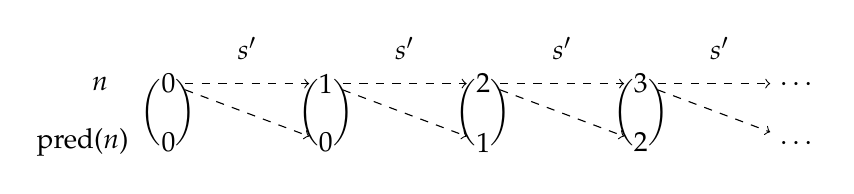
\begin{tikzpicture}
    \node at (-1, 0.75) {~~~$n$};
    \node at (-1, 0.0) {pred($n$)~~~};

    \node(c00) at (0, 0.0) {0};
    \node(c01) at (0, 0.75) {0};

    \node(c10) at (2, 0.0) {0};
    \node(c11) at (2, 0.75) {1};

    \node(c20) at (4, 0.0) {1};
    \node(c21) at (4, 0.75) {2};

    \node(c30) at (6, 0.0) {2};
    \node(c31) at (6, 0.75) {3};

    \node(c40) at (8, 0.0) {$\dots$};
    \node(c41) at (8, 0.75) {$\dots$};

    \draw[->, dashed] (c01) to (c11);
    \draw[->, dashed] (c01) to (c10);
    \draw[->, dashed] (c11) to (c21);
    \draw[->, dashed] (c11) to (c20);
    \draw[->, dashed] (c21) to (c31);
    \draw[->, dashed] (c21) to (c30);
    \draw[->, dashed] (c31) to (c41);
    \draw[->, dashed] (c31) to (c40);
    
    \node at (1, 1.2) {$s'$};
    \node at (3, 1.2) {$s'$};
    \node at (5, 1.2) {$s'$};
    \node at (7, 1.2) {$s'$};
    
    \node at (0, 0.375) {$\left(\begin{matrix}~~\\~~\end{matrix}\right)$};
    \node at (2, 0.375) {$\left(\begin{matrix}~~\\~~\end{matrix}\right)$};
    \node at (4, 0.375) {$\left(\begin{matrix}~~\\~~\end{matrix}\right)$};
    \node at (6, 0.375) {$\left(\begin{matrix}~~\\~~\end{matrix}\right)$};
\end{tikzpicture}
\end{center}

Cette représentation nous permet enfin d'écriture le lambda-terme pred :
$$\operatorname{pred} = \lambda n.~\operatorname{snd}~\left(n~s'~z'\right)$$

Vérifions que le résultat de pred sur un entier de Church donne bien l'entier de Church précédent. On suppose donc que $n$ est de la forme 
$$\lambda S.~ \lambda z.~\underbrace{S~(S~\dots(S}_\text{$n$ fois}~z))$$
Alors le calcul de $(n~s'~z')$ applique $n$ fois $s'$ à $(z')$, ce qui renvoie donc un couple $(n, n-1)$ selon la définition de $s'$ et $'z$. Enfin, on applique $\operatorname{snd}$ ce qui redonne $n-1$ sous forme d'entier de Church !

\begin{example}
    Calcul détaillé :
    \begin{equation*}
    \begin{aligned}
        \operatorname{pred}~2&=\underline{\left(\lambda n.~\operatorname{snd}~\left(n~s'~z'\right)\right) ~2}\\
        &\longrightarrow \operatorname{snd}~\left(2~s'~z'\right)\\
        &=\operatorname{snd}~\left(\underline{\underline{\left(\lambda S.~\lambda z.~ S(S~z)\right)~s'}~z'}\right)\\
        &\longrightarrow^* \operatorname{snd}~\left(s'~(s'~z')\right)\\
        \text{Or, séparément : }s'~z' &= \underline{\left(\lambda n.~\operatorname{tuple}_2~\left(\operatorname{succ}~\left(\operatorname{fst}~n\right)\right)~\left(\operatorname{fst}~n\right)\right)~\left(\operatorname{tuple}_2~0~0\right)}\\
        &\longrightarrow \operatorname{tuple}_2~\left(\operatorname{succ}~\left(\underline{\operatorname{fst}~\left(\operatorname{tuple}_2~0~0\right)}\right)\right)~\left(\underline{\operatorname{fst}~\left(\operatorname{tuple}_2~0~0\right)}\right)\\
        &\longrightarrow^* \operatorname{tuple}_2~\left(\underline{\operatorname{succ}~0}\right)~0\\
        &\longrightarrow^*\operatorname{tuple}_2~1~0 \equiv_\beta (1, 0)\\
        \text{Similairement : }s' ~(s'~z') &\equiv_\beta s'~(1, 0) \equiv_\beta (2, 1)\\
        \text{Ce qui donne enfin : } \operatorname{pred}~2&\equiv_\beta\operatorname{snd}~(2, 1)\equiv_\beta 1
    \end{aligned}
    \end{equation*}

    On a bien calculé le prédécesseur de 2, c'est 1
\end{example}

Et grâce à cela, on peut définir la soustraction.
$$\operatorname{sub} = \lambda n.~\lambda m.~m~\operatorname{pred}~n$$

Ce $\lambda$-terme calcule bien $n-m$ \underline{sous condition que $n\ge m$}. En effet, puisqu'on a essentiellement imposé que $\operatorname{pred}~0\equiv_\beta 0$, cela a donné que si $m < n$, on aura $\operatorname{sub}~n~m\equiv_\beta 0$.

Ceci concept s'applique aussi aux listes finies en construisant des couples qui contiennent la liste, et sa queue (voire même sa tête). Cette-fois ci, la fonction pred devient << tail >>. Et similairement au fait que le prédécesseur de 0 soit 0, la queue de la liste vide est la liste vide.

\subsection{Récursivité avec des points fixes}

Jusque là, nous avons vu comment représenter plein de types d'objets différents avec des $\lambda$-termes. Mais quelque chose nous embête encore : on ne peut pas faire de boucles, ni de récursivité, ce qui fait que, à ce que l'on sache, le $\lambda$-calcul n'est pas Turing-complet.

Dans cette partie, on raisonne sur la récursivité, ce qui permettra de faire des boucles. Il faut que l'on comprenne comment fonctionne la récursive sur le plan calculatoire. Regardons de plus près en OCaml ce qu'est une fonction récursive :

$$\verb|let |\underline{\texttt{rec}}\verb| f x = if x <= 0 then () else f (x - 1)|$$

Le mot-clé \verb|rec| permet d'accéder à la variable \verb|f| dans sa propre définition. Voilà déjà une différence avec le lambda-calcul : on ne peut pas faire référence à la $\lambda$-abstraction dans laquelle on se situe, parce qu'une fois qu'elle est appliquée, le lambda et le paramètre disparaîssent, ce qui empêche toute sorte de récursivité.

Si on veut espérer pouvoir faire des appels récursifs, il faut donc passer la fonction \verb|f| en argument dans elle-même. Tentons donc de reproduire cela en OCaml (et donc, sans utiliser le mot-clé \verb|rec|) :
$$\verb|let f_rec self x = if x <= 0 then () else self (x - 1)|$$

Le type de cette fonction est
$$\underbrace{\texttt{(int -> unit)}}_{\texttt{self}}\verb| -> |\underbrace{\underbrace{\texttt{int}}_{\tt{x}}\texttt{ -> unit}}_{\tt{f}}$$

C'est très prometteur ! Le type de \verb|self| semble être du même type que \verb|f| elle-même. Ainsi, il ne reste plus qu'à appliquer \verb|f_rec| à elle-même pour remplacer \verb|self| par \verb|f_rec|, ce qui donnera bien un appel récursif à la même fonction :
$$\verb|let f = |\color{red}\verb|f_rec f_rec|\color{black}$$

Aïe ! -- ça n'a pas fonctionné\dots voici l'erreur émise par OCaml sur le segment de code en rouge :
\begin{equation*}
\begin{aligned}
    &\verb|This expression has type (int -> unit) -> int -> unit|\\
           &\verb|    but an expression was expected of type int -> unit|\\
           &\verb|    Type int -> unit is not compatible with type int|\\
\end{aligned}
\end{equation*}

C'est une erreur de typage... bizarre. Rappelons-nous qu'il n'est pas possible d'appliquer une fonction à elle-même en OCaml. Et oui, si une telle fonction $h: \alpha \to \beta$ était appelée à elle même, ceci imposerait que $\alpha=\alpha\to\beta$ ce qui n'est pas possible, car autrement la fonction $h$ est de type
$$(\alpha \to \beta)\to\beta$$
mais encore
$$(((\dots) \to \beta) \to \beta)\to\beta$$
bref, un type infini, ce qui n'est pas autorisé par définition des types (nous y reviendrons plus tard).

\begin{remark}
    Dans certains langages de programmation, de tels types sont autorisés (par exemple dans le cadre du sous-typage). On noterai alors le type de la fonction $h$ comme ceci :
    $$h: \mu x.~x \to \beta$$
\end{remark}

Le problème qui fait qu'on ne peut pas << simplifier >> l'écriture d'une fonction récursive en OCaml découle du fait que le langage soit fortement typé. Mais, nous n'avons pas encore introduit le typage sur $(\lambda)$, et donc il est toujours parfaitement acceptable d'écrire 
$$\Delta = \lambda x.~x~x$$
Et ce genre d'écriture a parfois de drôles de comportements. Par exemple, lorsque nous avons introduit $\Delta$, nous avons vu que le terme $\Delta~\Delta$ n'avait pas de forme normale, car une $\beta$-réduction redonnait exactement le même terme (et donc qu'il divergeait).
$$\Delta~\Delta\longrightarrow\Delta$$
Le $\lambda$-terme $\Delta$ est appelé << le combinateur divergent >>. Pourrait-on utiliser un lambda-terme similaire pour implémenter les fonctions récursives ? Il se trouve que oui ! Le combinateur $\Delta$ a une généralisation utile justement pour cela :

\begin{definition}
    $$Y = \lambda f.~\left(\lambda x.~f~(x~x)\right)~\left(\lambda x.~f~(x~x)\right)$$
    Ce $\lambda$-terme est appelé << combinateur paradoxal >> (dû aux travaux de Haskell Curry sur la logique).
    
    Il est souvent noté $Y$ dans la littérature, mais aussi parfois noté $\operatorname{fix}$ (en raison d'une propriété que nous allons voir dans un instant).
\end{definition}

Le terme $\operatorname{fix}$ ressemble un peu au combinateur divergent $\Delta$, et il est difficile de comprendre ce qu'il fait lorsque l'on applique à un terme $f$. Mais il vérifie une propriété très intéressante qui nous permettra de faire marcher les fonction récursives de la manière que nous avons essayé avec une fonction OCaml.

\begin{theorem}
    $Y$ est un \textit{combinateur de point fixe}. Autrement dit, pour tout terme $f$ :
    $$f~\left(Y~f\right) \equiv_\beta Y~f$$

    C'est-à-dire, $Y~f$ est un point fixe de $f$.

    \begin{preuve}
    On vérifie manuellement le résultat par $\beta$-réduction :
    \begin{equation*}
    \begin{aligned}
        Y~f&=\underline{\left(\lambda f.~\left(\lambda x.~f~(x~x)\right)~\left(\lambda x.~f~(x~x)\right)\right)~f}\\
        &\longrightarrow \underline{\left(\lambda x.~f~(x~x)\right)~\left(\lambda x.~f~(x~x)\right)}\\
        &\longrightarrow f~(\underbrace{\left(\lambda x.~f~(x~x)\right)~\left(\lambda x.~f~(x~x)\right)}_{Y~f})\\
        &=f~\left(Y~f\right)
    \end{aligned}
    \end{equation*}

    d'où $f~\left(Y~f\right) \equiv_\beta Y~f$.
    \end{preuve}
\end{theorem}

Quel intérêt ce terme a-t-il ? Lorsque que j'ai un terme de la forme $Y~f$, alors il est en réalité équivalent à $f~(Y~f)$, mais donc aussi à $f~(f~(Y~f))$, donc à $f~(f~(f~(Y~f)))$, et en continuant un nombre arbitraire de fois :
$$Y~f \equiv_\beta \underbrace{f~(f~(\dots (f~(f}_\text{répétition de $f$}~(Y~f)))))$$

On observe alors qu'utiliser $Y~f$ revient à directement à appeler $f$ avec $Y~f$ en paramètre pour un usage prochain dans la fonction $f$, qui lui aura aussi le même effet, etc... C'est exactement le principe de la récursivité !

Ainsi, si je veux définir une fonction récursive $f$, je vais d'abord définir une fonction $f_\text{Rec}$ non-récursive qui se prendra \textit{d'abord en argument << elle-même >>}, qu'on désignera par $\text{Self}$, puis qui prendra les mêmes arguments que $f$. $f_\text{Rec}$ utilisera Self pour s'appeler elle-même grâce à $Y$, car on posera à la fin :
$$f=Y~f_\text{Rec}$$

Tentons cela ! Pour commencer, un exemple simple : on va écrire un lambda-terme qui agit comme une fonction qui fait de décompte à partir d'un entier $n$ de Church jusqu'à 0. Appelons-là Countdown.

\begin{remark}
    Avant de commencer, je me donne temporairement des lambda-termes que je vais utiliser pour coder cette fonction.
    \begin{itemize}
        \item Une constante << unit >> qui représente le tuple vide.
        \item Un $\lambda$-terme IsZero qui prend un entrée un entier de Church et renvoie un booléen de Church, valant true si l'entier était nul, false sinon. Ce lambda-terme n'est pas magique, il est défini par :
        $$ \lambda n.~n~\left(\lambda\verb|_|.~\operatorname{false}\right)~\operatorname{true} $$
    \end{itemize}
\end{remark}

\begin{enumerate}
    \item D'abord, on définit une fonction $\text{Countdown}_\text{Rec}$ qui prend une fonction Self en argument, puis l'entier initial
    $$\text{Countdown}_\text{Rec}=\lambda\text{Self}.~\lambda n.~ (???)$$
    \item On peut alors écrire le corps de la fonction en vérifiant grâce à if si l'entier est nul. Dans ce cas, je retourne unit, sinon, je recommence avec $n-1$ avec un appel récursif.
    $$\text{Countdown}_\text{Rec}=\lambda\text{Self}.~\lambda n.~ 
    \operatorname{if}~(\text{IsZero}~n)~\operatorname{unit}~\left(\operatorname{Self}~\left(\operatorname{pred}~n\right)\right)
    $$
    \item J'achève la définition de mon lambda-terme Countdown avec le combinateur de point fixe :
    $$\text{Countdown} = Y~\text{Countdown}_\text{Rec}$$
    \item Vérifions donc l'exécution de ce terme avec 5 comme entrée initiale !
    \begin{equation*}
    \begin{aligned}
        \text{Countdown}~5&=\left(Y~\text{Countdown}_\text{Rec}\right)~5\\
        &\equiv_\beta \left(\text{Countdown}_\text{Rec} \left(Y~\text{Countdown}_\text{Rec}\right)\right)~5\\
        &= \text{Countdown}_\text{Rec}~\text{Countdown} ~5\\
        &=\underline{\underline{\left(\lambda\text{Self}.~\lambda n.~ 
        \operatorname{if}~(\text{IsZero}~n)~\operatorname{unit}~\left(\operatorname{Self}~\left(\operatorname{pred}~n\right)\right)\right)~\text{Countdown}}~5}\\
        &\longrightarrow^* \operatorname{if}~(\text{IsZero}~5)~\operatorname{unit}~(\text{Countdown}~(\underline{\operatorname{pred}~5}))\\
        &\longrightarrow^* \operatorname{if}~(\underline{\text{IsZero}~5})~\operatorname{unit}~(\text{Countdown}~4)\\
        &\longrightarrow^* \operatorname{if}~\operatorname{false}~\operatorname{unit}~(\text{Countdown}~4)\\
        &\equiv_\beta \text{Countdown}~4\\
        &\equiv_\beta \operatorname{if}~(\underline{\text{IsZero}~4})~\operatorname{unit}~(\text{Countdown}~3)\\
        &\equiv_\beta \text{Countdown}~3\\
        &\equiv_\beta \text{Countdown}~2\\
        &\equiv_\beta \text{Countdown}~1\\
        &\equiv_\beta \text{Countdown}~0\\
        &\longrightarrow^* \operatorname{if}~(\underline{\text{IsZero}~0})~\operatorname{unit}~(\text{Countdown}~0)\\
        &\longrightarrow^* \operatorname{if}~\operatorname{true}~\operatorname{unit}~(\text{Countdown}~0)\\
        &\longrightarrow^*\operatorname{unit}
    \end{aligned}
    \end{equation*}

    Cela a bien donné le décompte de 5 à 0, puis unit. C'est exactement ce que l'on attendait !
\end{enumerate}

\begin{example}
    Un autre exemple plus compliqué cette fois-ci : on va définir la fonction factorielle de manière récursive. On l'appelle $\text{fact}$
    $$\text{fact}_\text{Rec} = \lambda \text{Self}.~\lambda n.~\text{if}~(\text{IsZero}~n)~1~(\text{mul}~n~(\text{Self}~(\text{pred}~n)))$$
    Puis on achève avec :
    $$\text{fact} = Y~\text{fact}_\text{Rec}$$
    
    Essayons avec 6 :
    \begin{equation*}
    \begin{aligned}
        \text{fact}~6&\equiv_\beta \text{fact}_\text{Rec}~\text{fact}~6\\
        &\longrightarrow^* \text{if}~(\text{IsZero}~6)~1~(\text{mul}~6~(\text{fact}~(\underline{\text{pred}~6})))\\
        &\longrightarrow^* \text{if}~(\underline{\text{IsZero}~6})~1~(\text{mul}~6~(\text{fact}~5))\\
        &\longrightarrow^* \text{if}~\text{false}~1~(\text{mul}~6~(\text{fact}~5))\\
        &\longrightarrow^* \text{mul}~6~(\underline{\text{fact}~5})\\
        &\equiv_\beta \text{mul}~6~(\text{mul}~5~(\underline{\text{fact}~4}))\\
        &\equiv_\beta \text{mul}~6~(\text{mul}~5~(\text{mul}~4~(\underline{\text{fact}~3})))\\
        &\equiv_\beta \text{mul}~6~(\text{mul}~5~(\text{mul}~4~(\text{mul}~3~(\underline{\text{fact}~2}))))\\
        &\equiv_\beta \text{mul}~6~(\text{mul}~5~(\text{mul}~4~(\text{mul}~3~(\text{mul}~2~(\underline{\text{fact}~1})))))\\
        &\equiv_\beta \text{mul}~6~(\text{mul}~5~(\text{mul}~4~(\text{mul}~3~(\text{mul}~2~(\text{mul}~1~(\underline{\text{fact}~0}))))))\\
        &\equiv_\beta \text{mul}~6~(\text{mul}~5~(\text{mul}~4~(\text{mul}~3~(\text{mul}~2~(\text{mul}~1~1)))))\\
        &\longrightarrow^* 720
    \end{aligned}
    \end{equation*}
\end{example}

\begin{example}
    Fibonacci récursif
    \begin{equation*}
    \begin{aligned}
        \text{fib}_\text{Rec} =~& \lambda \text{Self}.~\lambda{n}.\\
        &~~\text{if}~(\text{IsZero}~n)~0~(\\
        &~~~~\text{if}~(\text{IsZero}~(\text{pred}~n))~1~(\\
        &~~~~~~\text{add}~(\text{Self}~(\text{pred}~n))~(\text{Self}~(\text{pred}~(\text{pred}~n)))\\
        &~~~~)\\
        &~~)\\
    \end{aligned}
    \end{equation*}
    $$\text{fib} = Y~\text{fib}_\text{Rec}$$
\end{example}

\section{Le lambda-calcul simplement typé}

Après avoir étudié de lambda-calcul de manière plus ou moins détaillée, il est grand temps de faire le rapprochement avec les langages de programmation et le typage. Ceci va nous prendre quelques temps car il va falloir redéfinir une nouvelle syntaxe pour les types, et tous les autres outils que l'on va utiliser pour le typage.

La première chose que l'on va faire est de choisir une stratégie de réduction qui correspond à l'évaluation dans la plupart des langages de programmation (notamment OCaml). En OCaml, lorsqu'une fonction est appelée, on évalue d'abord tous les arguments qu'elle reçoit, puis on effectue l'application de la fonction. Autrement dit, on ne peut passer dans une fonction que des termes qui ont déjà été totalement évalués : ce sont des valeurs, et non des expressions. Mettons la main sur cette notion :

\begin{definition}
    On définit l'ensemble des valeurs $V\subset \Lambda$ comme ensemble inductif :
    $$ v := \lambda x.~e$$
    ... où $e$ désigne les lambda-termes quelconques.

    Autrement dit, une valeur est une $\lambda$-abstraction (une fonction).
\end{definition}

Grâce à cette notion de << valeur >>, on peut détailler la définition de la stratégie que l'on va utiliser. C'est la stratégie {\scshape{call-by-value}}. Lorsque nous avons défini la relation de $\beta$-réduction, nous avions en réalité utilisé la stratégie appelée {\scshape{full}-$\beta$}, qui autorise la réduction de n'importe quel rédex.

Cependant, la stratégie {\scshape{call-by-value}} est plus complexe, et il faut imposer des conditions sur un rédex pour pouvoir l'évaluer. Pour pouvoir représenter ces conditions, nous allons utliser, comme en logique propositionelle, des règles d'inférences.

\begin{definition}
    L'évaluation par {\scshape{call-by-value}} (appel par valeur) est définie par les règles suivantes :
    $$\infer[(\text{\scshape{E-App1}})] {t_1~t_2 \longrightarrow t_1'~t_2}{t_1\longrightarrow t_1'}$$
    $$\infer[(\text{\scshape{E-App2}})] {v_1~t_2 \longrightarrow v_1~t_2'}{t_2\longrightarrow t_2'}$$
    $$\infer[(\text{\scshape{E-Call}})] {(\lambda x.~e)~v\longrightarrow e\left[x\leftarrow v\right]}{}$$
\end{definition}

Les deux premières règles permettent tout d'abord d'évaluer les arguments à un $\lambda$-terme dans l'ordre. En effet, la première évalue la fonction jusqu'à ce qu'elle soit une valeur. Ensuite, la deuxième règle évalue les arguments jusqu'à ce qu'ils deviennent des valeurs. Enfin, la dernière et plus importante des règles, détecte lorsqu'il y a une lambda-abstraction appliqué à une valeur, et performe la réduction du rédex.

Remarquons un autre point important : les variables libres de sont pas des valeurs. En effet, si je ne sais pas ce qu'est une variable, je peux pas l'évaluer. On va donc travailler sur un sous-ensemble de termes qui vérifient une propriété qui empêche d'être bloqué par des variables libres.

\begin{definition}
    Un terme $e\in\Lambda$ est dit << fermé >> s'il ne contient aucune variable libre : $\text{FV}(e)=\emptyset$
\end{definition}

\begin{example}
    Juste pour bien comprendre, regardons l'évaluation du terme suivant, avec $y\in V$ :
    \begin{equation*}
    \begin{aligned}
        \text{app}~\text{id}~(\text{id}~y) &\equiv_\beta (\lambda f.~\lambda x.~f~x)~(\lambda t.~t)~((\lambda t.~t)~y)\\
        &\,_{(1)}\longrightarrow (\lambda x.~(\lambda t.~t)~x)~((\lambda t.~t)~y)&~~~~~~~\text{par ({\scshape{E-App1}}) puis (\scshape{E-Call})}\\
        &\,_{(2)}\longrightarrow (\lambda x.~(\lambda t.~t)~x)~y&~~~~~~~\text{par ({\scshape{E-App2}}) puis (\scshape{E-Call})}\\
        &\,_{(3)}\longrightarrow (\lambda t.~t)~y&~~~~~~~\text{par (\scshape{E-Call})}\\
        &\,_{(4)}\longrightarrow y\in V&~~~~~~~\text{par (\scshape{E-Call})}\\
    \end{aligned}
    \end{equation*}
    
    A chaque étape de cette évaluation (lorsqu'il y a une flèche à gauche d'un terme), il se cache un arbre d'évaluation terminé :
    \begin{enumerate}
        \item
        $$\infer[(\text{\scshape{E-App1}})] {
        (\lambda f.~\lambda x.~f~x)~(\lambda t.~t)~((\lambda t.~t)~y)\longrightarrow (\lambda x.~(\lambda t.~t)~x)~((\lambda t.~t)~y)
        }
        {
            \infer[(\text{\scshape{E-Call}})]
            {(\lambda f.~\lambda x.~f~x)~(\lambda t.~t)\longrightarrow (\lambda x.~(\lambda t.~t)~x)}
            {}
        }$$

        \item $$
        \infer[(\text{\scshape{E-App2}})]
        {
            (\lambda x.~(\lambda t.~t)~x)~((\lambda t.~t)~y) \longrightarrow (\lambda x.~(\lambda t.~t)~x)~y
        }
        {
            \infer[(\text{\scshape{E-Call}})]
            {
                ((\lambda t.~t)~y)\longrightarrow y
            }
            {}
        }
        $$

        \item $$
            \infer[(\text{\scshape{E-Call}})]
            {
                (\lambda x.~(\lambda t.~t)~x)~y\longrightarrow(\lambda t.~t)~y
            }
            {}
        $$

        \item $$
            \infer[(\text{\scshape{E-Call}})]
            {
                (\lambda t.~t)~y \longrightarrow y
            }
            {}
        $$
    \end{enumerate}

    Ce qui prouve enfin que $\text{app}~\text{id}~(\text{id}~y)\equiv_\beta y$
\end{example}

Avec tout cela en place, il est logique de vouloir imposer que la réduction itérée d'un $\lambda$-terme initial soit une valeur $v\in V$. En effet, certain termes, comme $\Delta~\Delta$ divergent, ce qui ne modélise pas vraiment une évaluation selon celle d'OCaml.

Le problème se pose donc de la manière suivante : étant donné un terme initiale $e\in\Lambda$, \textbf{quelle condition suffisante peut-on imposer pour que son évaluation donne une valeur, et ne reste pas bloquée ?}

\textit{Spoiler alert} : il suffise qu'il soit << bien typé >>.

\subsection{Extension de ($\lambda$) avec des types}

Afin de construire le << typage >> sur $(\lambda)$, il faut tout d'abord définir les types.

\begin{definition}
    Etant donné un ensemble $\mathcal{V}'$ de variables, n définie l'ensemble $\mathcal{T}$ des types par :
    \begin{equation*}
    \begin{aligned}
        \tau &:= x\\
        &\mid~\tau\to\tau\\
    \end{aligned}
    \end{equation*}
\end{definition}

Ainsi, un type est soit une variable $\alpha\in\mathcal{V}'$, soit le type d'une fonction d'un type $\tau_1$ vers un type $\tau_2$, qui sera noté $\tau_1\to\tau_2$. Généralement, on utilise des lettres grecques pour les types, et des lettres de l'alphabet latin pour les variables d'un terme.

On va maintenant étendre la syntaxe du lambda-calcul pour pouvoir utiliser ces types dans des $\lambda$-termes.

\begin{definition}
    Le \textbf{lambda-calcul simplement typé}, noté $\left(\lambda_\rightarrow\right)$, est l'ensemble des termes $\Lambda_\rightarrow$ défini par :
    \begin{equation*}
    \begin{aligned}
        e &:= x\\
        &|~\lambda x: \tau.~e\\
        &|~e~e\\
    \end{aligned}
    \end{equation*}

    On a juste rajouté une syntaxe pour l'annotation de type d'une variable liée dans une $\lambda$-abstraction.
\end{definition}

\begin{example}
    On peut maintenant traduire certains lambda-termes dans le lambda-calcul simplement typé.
    $$\text{id}=\lambda x: \alpha.~x$$
    $$\text{app}=\lambda f:\alpha\to\beta.~\lambda x:\alpha.~f~x$$
    $$\text{true}=\lambda x: \alpha.~\lambda y:\alpha.~y$$
\end{example}

Cette syntaxe nous a essentiellement permis de << typer >> les variables d'une $\lambda$-abstraction. Cependant, rien ne nous empêche d'écrire un terme comme celui-ci
$$\lambda f:\tau\to\tau.~f~f$$
sans vérifie que $f~f$ ne soit << bien typé >> lui aussi. Pour l'instant, << bien typé >> ne veut pas dire grand chose, donc nous allons le définir.

Peut-être que vous avez déjà entendu parler de la correspondance (ou isomorphisme) de Curry-Howard ! Ce théorème stipule que typer une fonction est rigoureusement équivalent à prouver une formule propositionelle. Ainsi, comme pour la logique propositionelle, nous allons nous appuyer sur des arbres de dérivation pour prouver qu'un $\lambda$-terme ait un certain type.

Rappelez-vous que lorsque l'on travaille avec des arbres de preuve de formules, on effectue un travail syntaxique sur des \textit{prémisses}, selon des règles d'inférences données. Un séquent est constitué de deux choses :
\begin{itemize}
    \item un \textit{contexte} noté $\Gamma$, qui stocke les formules logiques dont une certain valuation $\nu$ est modèle.
    \item un \textit{but} noté $\varphi$ qui est la formule à satisfaire avec cette même valuation ($\varphi$ est conséquence logique du contexte)
\end{itemize}
Un telle séquent est donc notée :
$$\Gamma \vdash \varphi$$

Ici, nous allons redéfinir ce qu'est un contexte exactement, puis redéfinir un séquent dans le contexte du typage.

\begin{definition}
    Un contexte $\Gamma$ est une collection de renseignements sur les types des variables connues. On le définit par induction :
    \begin{equation*}
    \begin{aligned}
        \Gamma &:=\emptyset\\
        &|~\Gamma,~x:\tau\\
    \end{aligned}
    \end{equation*}

    On peut le voir comme une liste de typages de variables -- autrement dit, un élément de $\text{List}(\mathcal{V}\times\mathcal{T})$.
\end{definition}

\begin{definition}
    Un séquent est constitué d'un contexte $\Gamma$, et du typage d'un lambda-terme $e\in\Lambda_\rightarrow$ par un type $\tau\in\mathcal{T}$, qui se note :
    $$\Gamma\vdash e:\tau$$
\end{definition}

Il ne nous reste plus qu'à définir nos règles d'inférences pour pouvoir construire des arbres de dérivation, ce qui << prouvera >> qu'un $\lambda$-terme est d'un type $\tau$ donné. Cette preuve, comme en logique propositionelle, sera sous la forme d'un arbre de dérivation terminé, c'est-à-dire que toutes les feuilles n'aient aucun séquent.

Comment choisir nos règles d'inférences ? Et bien, puisque nous avons trois formes de $\lambda$-termes différents, nous allons construire trois règles qui nous permettront de typer n'importe quel terme. Détaillons donc comment obtenir ces règles.

\begin{itemize}
    \item \underline{Cas n°1} : $e$ est une variable $x$. Comment prouver que $x:\tau$ ? Et bien, la seule manière de le prouver est de vérifier que l'information $x:\tau$ soit bien présente dans le contexte $\Gamma$. D'où la première règle d'inférence :
    $$
    \infer[(\text{\scshape{T-Ax}})] 
    {\Gamma,~x:\tau\vdash x:\tau}{}
    $$
    
    \begin{remark}
        Cette règle d'inférence correspond à la règle ({\scshape{Ax}}) en logique propositionelle.
    \end{remark}

    \item \underline{Cas n°2} : $e$ est une application $f~a$. Intuitivement, il faut que la fonction soit d'un type $\alpha\to\beta$, et que sont argument soit de type $\alpha$, ce qui renverrait donc un terme de type $\beta$. Ainsi, pour montrer que $f~a:\beta$, on utilise des séquents en hypothèses (appelées << prémisses >>), qui montrent que $f:\alpha\to\beta$, et aussi que $a:\alpha$.
    $$
    \infer[(\text{\scshape{T-App}})]
    {\Gamma \vdash f~a:\beta}
    {\Gamma\vdash f:\alpha\to\beta & \Gamma\vdash a:\alpha}
    $$
    
    \begin{remark}
        Cette règle correspond à la règle ($\rightarrow_e$) -- le modus ponens.
    \end{remark}

    \item \underline{Cas n°3} : $e$ est une $\lambda$-abstraction de la forme $(\lambda x:\alpha.~b)$. Pour déduire le type d'une telle fonction, il suffit d'ajouter $x:\alpha$ dans le contexte, et de déduire le type de $b:\beta$, ce qui donnera au total le type $\alpha\to\beta$ :
    $$
    \infer[(\text{\scshape{T-Abs}})]
    {\Gamma\vdash(\lambda x:\alpha.~b):\alpha\to\beta}
    {\Gamma,~x:\alpha\vdash b:\beta}
    $$

    \begin{remark}
        Cette règle correspond à la règle ($\rightarrow_i$).
    \end{remark}
\end{itemize}

Pour résumer, les règles d'inférence de typage sont donc :
\begin{definition}
    Pour $e\in\Lambda_\rightarrow$ et $\tau\in\mathcal{T}$ on prouve que $\Gamma\vdash e:\tau$ avec les règles suivantes :
    $$
    \infer[(\text{\scshape{T-Ax}})] 
    {\Gamma,~x:\tau\vdash x:\tau}{}
    $$
    $$
    \infer[(\text{\scshape{T-Abs}})]
    {\Gamma\vdash(\lambda x:\alpha.~b):\alpha\to\beta}
    {\Gamma,~x:\alpha\vdash b:\beta}
    $$
    $$
    \infer[(\text{\scshape{T-App}})]
    {\Gamma \vdash f~a:\beta}
    {\Gamma\vdash f:\alpha\to\beta & \Gamma\vdash a:\alpha}
    $$
\end{definition}

\begin{example}
    Prouvons que $\text{app}:(\alpha\to\beta)\to\alpha\to\beta$
    $$
    \infer[(\text{\scshape{T-Abs}})]
    {
        \vdash(\lambda f:\alpha\to\beta.~\lambda x:\alpha.~f~x):(\alpha\to\beta)\to\alpha\to\beta
    }
    {
        \infer[(\text{\scshape{T-Abs}})]
        {
            f:\alpha\to\beta\vdash(\lambda x:\alpha.~f~x):\alpha\to\beta
        }
        {
            \infer[(\text{\scshape{T-App}})]
            {
                f:\alpha\to\beta, x: \alpha\vdash f~x:\beta
            }
            {
                \infer[(\text{\scshape{T-Ax}})]
                {\underline{f:\alpha\to\beta}, x: \alpha\vdash f:\alpha\to\beta}
                {}
                &
                \infer[(\text{\scshape{T-Ax}})]
                {f:\alpha\to\beta, \underline{x: \alpha}\vdash x:\alpha}
                {}
            }
        }
    }
    $$

    L'arbre de dérivation étant bien terminé, on conclut avec le résultat du typage.

    $$\text{app}:(\alpha\to\beta)\to\alpha\to\beta$$
\end{example}

\begin{theorem}
    \textbf{Inversibilité}

    Les règles d'inférences sont inversibles. Plus précisément
    \begin{enumerate}
        \item Si $\Gamma \vdash x:\tau$, alors $(x:\tau)\in\Gamma$.
        \item Si $\Gamma \vdash (\lambda x:\alpha.~b):\tau$, alors $\tau=\alpha\to\beta$ (avec un certain $\beta\in\mathcal{T}$), et $\Gamma, x:\alpha\vdash b:\beta$
        \item Si $\Gamma\vdash e_1~e_2:\beta$, alors il existe un type $\alpha$ tel que $\Gamma\vdash e_1:\alpha\to\beta$, et $\Gamma\vdash e_2:\alpha$
    \end{enumerate}

    \begin{preuve}
        Directe par lecture des règles d'inférences. Il n'y a presque rien à dire.
    \end{preuve}
\end{theorem}

Ce théorème est utilisé si souvent que ce n'est visiblement parfois pas la peine de le mentionner (ce qui m'a bien embêté lorsque je ne comprenais pas la preuve d'un des lemmes que nous allons montrer).

\subsection{Sécurité = avancement + préservation}

En quoi ces mécanismes nous permettent-ils de déduire des propriété d'évaluation sur les lambda-termes simplement typés ? Nous avons défini la relation de typage avec des règles d'inférences, et de même, l'évalution (sous la stratégie d'appel par valeur) avec d'autres règles d'inférences. De ce fait, nous allons débloquer le pouvoir de faire jouer les deux ensemble pour appliquer des propriétés de typage sur des évaluations, et aussi, appliquer des propriétés de réduction sur le typage.

Le système de type que l'on a défini jusqu'ici vérifie une propriété très basique mais tout autant essentielle : on l'appelle la << \textit{sécurité} >> (safety). Cette propriété stipule grossièrement que les termes typés << ne vont pas mal tourner >> lorsqu'on les évaluera. Plus précisément, par << mal tourner >>, on veut entendre qu'un terme ne sera jamais bloqué pendant l'évaluation, et qu'il terminera toujours par une valeur $v\in V$.

Cette propriété de << sécurité >> se décompose en deux invariants :
\begin{itemize}
    \item \textbf{l'avancement} : un terme bien typé n'est pas bloqué -- c'est soit une valeur, soit c'est un terme qui peut effectuer une étape d'évaluation (selon la stratégie {\scshape{call-by-value}}).
    \item \textbf{la préservation} : si un terme bien typé effectue une étape d'évaluation, le terme résultant est aussi bien typé.
\end{itemize}

On voit bien intuitivement que ces invariants montrent qu'un terme bien typé sera à un certain moment évalué en une valeur finale.

Dans cette partie on s'intéresse à la preuve de la sécurité.

\subsubsection{Quelques lemmes}

Avant d'attaquer la preuve, on va se servir de quelques lemmes qui nous faciliteront certains raisonnements.

Le premier lemme permet d'ajouter des variables dans un contexte sans affecter le résultat du typage.

\begin{lemma}
    \textbf{Affaiblissement}

    Soit $x$ une variable telle que $x\notin\Gamma$. Alors
    $$\Gamma\vdash t:\tau\implies \Gamma, x:\alpha\vdash t:\tau$$

    L'ajout de $x:\alpha$ dans le contexte permet de prouver la même chose sur le type de $t$.
\end{lemma}

Si l'ou voulait être le plus rigoureux, il faudrait montrer que les preuves de typages sont stable par permutation du contexte. Je passe sous le tapis ce détail qui n'est pas trop intéressant, et je m'autorise à interchanger les variables dans un contexte, ou à extraires des sous-contextes à partir d'un contexte, sans me soucier de l'ordre dans lequel ses variables sont écrites.

Le second va permettre de déduire la forme d'un terme étant donné son type. Puisque notre système de typage est pour l'instant très simple, ce lemme est plutôt court. 

\begin{lemma}
    \textbf{Lemme des formes canoniques}
    
    Soit $v\in V$ une valeur de type $\tau_1\to\tau_2$. Alors $\exists e\in\Lambda_\rightarrow~|~v=\lambda x:\tau_1.~e$

    Autrement dit, une valeur dont le type est celui d'une abstraction est elle-même une abstraction.

    \begin{preuve}
    Si $v$ est une valeur, alors, par définition des valeurs $V$, $v$ s'écrit comme 
    $$v=\lambda x:\alpha.~e$$
    avec $e\in\Lambda_\rightarrow$ et $\alpha\in\mathcal{T}$.
    
    De plus, on sait que $v:\tau_1\to\tau_2$, donc l'arbre de preuve pour $v$ s'écrit :
    $$\infer[(\text{\scshape{T-Abs}})]{\Gamma\vdash(\underbrace{\lambda x:\tau_1.~e}_v):\tau_1\to\tau_2}{\dots}$$
    ce qui impose $\lambda x: \tau_1.~e=\lambda x:\alpha.~e$, donc $\alpha = \tau_1$.
    D'où $v=\lambda x:\tau_1~e$.
    \end{preuve}
\end{lemma}

Le lemme suivant est plus délicat et va nous permettre de conserver des propriété de typages après une $\beta$-réduction. Pour cela, il faut montrer que l'opération de substitution conserve les types.

\begin{lemma}
    \textbf{Stabilité par substitution}

    $$\Gamma,x:\sigma\vdash t:\tau~~\text{et}~~\Gamma\vdash\ s:\sigma\implies\Gamma\vdash t\left[x \leftarrow s\right]:\tau$$

    Autrement dit : si en sachant que $x:\sigma$, on peut prouver que $t:\tau$, et qu'on peut aussi prouver que $s:\sigma$, alors on peut prouver aussi que la substitution de $x$ par $s$ dans $t$ est du même type que $t$.
\end{lemma}

La preuve est trop grande donc je suis obligé de la sortir de la boîte du théorème.

\textbf{Preuve} : Puisque $\Gamma,x:\sigma\vdash t:\tau$, on a donc un arbre de preuve terminé sur lequel on va effectuer une induction structurelle.

\begin{itemize}
    \item \underline{Cas ({\scshape{T-Ax}})} : Si la première règle utilisée est ({\scshape{T-Ax}}), alors l'arbre de dérivation est de la forme
    $$\infer[(\text{{\scshape{T-Ax}}})]{\Gamma, x:\sigma, \dots, \underline{z:\tau}, \dots \vdash z:\tau}{}$$

    avec $t=z\in\mathcal{V}$ une variable. Lorsque l'on effectue une substitution sur une variable, il y a deux sous-cas :
    \begin{itemize}
        \item \underline{$z=x$} : donc $z[x\leftarrow s] = s$. On veut donc avoir $\Gamma\vdash s:\tau$, mais on peut déduire que $\tau=\sigma$ par inversion, ce qui fait partie des hypothèses du lemme. OK.
        \item \underbar{$z\ne x$}, donc la substitution ne fait rien, et on veut montrer que $z: \tau$, ce qui déjà prouvé.
    \end{itemize}

    \item \underline{Cas ({\scshape{T-Abs}})} : on a donc 
    $$\infer[]{\Gamma, x:\sigma\vdash (\underbrace{\lambda y:\tau_1.~e}_t):\underbrace{\tau_1\to\tau_2}_\tau}{\infer{\Gamma, x:\sigma, y:\tau_1\vdash e:\tau_2}{\dots}}~~~~~\text{avec}~~~~~\begin{cases}
        t = \lambda y:\tau_1.~e\\
        \tau=\tau_1\to\tau_2\\
    \end{cases}$$

    On va supposer que $x\ne y$ et $y\notin \text{FV}(s)$, sinon on ne pourrait pas effectuer la substitution. Effectuons-là :
    $$(\lambda y:\tau_1.~e)\left[x\leftarrow s\right] = (\lambda y:\tau_1.~e\left[x\leftarrow s\right])$$

    Prouvons donc que $(\lambda y:\tau_1.~e\left[x\leftarrow s\right]):\tau_1\to\tau_2$.

    $$
    \infer[\text{(\scshape{T-Abs})}]{
        \Gamma\vdash (\lambda y:\tau_1.~e\left[x\leftarrow s\right]):\tau_1\to\tau_2
    }
    {
        \infer{\Gamma, y:\tau_1\vdash e\left[x\leftarrow s\right]:\tau_1\to\tau_2}{???}
    }
    $$

    Or, par affaiblissement :
    $$
        \Gamma, x:\sigma \vdash s:\sigma\implies \Gamma, x:\sigma, y:\tau_1 \vdash s:\sigma
    $$
    et puisque $$\Gamma, x:\sigma, y:\tau_1\vdash e:\tau_2$$
    on peut appliquer l'hypothèse d'induction sur $e$, on a que $$\Gamma, y:\tau_1\vdash e[x\leftarrow s]:\tau_2$$

    Ce qui complète l'arbre de preuve de $(\lambda y:\tau_1.~e\left[x\leftarrow s\right]):\tau_1\to\tau_2$.

    \item \underline{Cas ({\scshape{T-App}})} : l'arbre s'écrit donc
    $$
    \infer[\text{(\scshape{T-App})}]{
        \Gamma, x:\sigma\vdash \underbrace{t_1~t_2}_t:\underbrace{\tau_2}_\tau
    }
    {
        \infer{\Gamma, x:\sigma\vdash t_1 :\tau_1\to\tau_2}{\dots}
        &
        \infer{\Gamma, x:\sigma\vdash t_2 :\tau_1}{\dots}
    }
    ~~~~~\text{avec}~~~~~\begin{cases}
        t=t_1~t_2\\
        \tau = \tau_2\\
        \tau_1\in\mathcal{T}\\
    \end{cases}
    $$

    La substitution de $x$ par $s$ dans ce terme est $\left(t_1~t_2\right)[x\leftarrow s]=\left(t_1[x\leftarrow s]\right)~\left(t_2[x\leftarrow s]\right)$. Prouvons alors que le type est le même pour ce nouveau terme : $\Gamma\vdash \left(t_1[x\leftarrow s]\right)~\left(t_2[x\leftarrow s]\right):\tau_2$

    $$
    \infer[(\text{\scshape{T-App}})]
    {
        \Gamma\vdash \left(t_1[x\leftarrow s]\right)~\left(t_2[x\leftarrow s]\right):\tau_2
    }
    {
        \infer{\Gamma\vdash\left(t_1[x\leftarrow s]\right):\tau_1\to\tau_2}{???}
        &
        \infer{\Gamma\vdash\left(t_2[x\leftarrow s]\right):\tau_1}{???}
    }
    $$

    Il faut compléter les feuilles de cet arbre : on va le faire en appliquant l'hypothèse d'induction avec les sous-termes $t_1$ et $t_2$. En effet, les hypothèses pour l'appliquer sont déjà remplies :
    $$\begin{cases}
        \Gamma, x:\sigma\vdash t_1 :\tau_1\to\tau_2\\
        \Gamma \vdash s:\sigma 
    \end{cases}\implies \Gamma\vdash\left(t_1[x\leftarrow s]\right):\tau_1\to\tau_2$$
    $$\begin{cases}
        \Gamma, x:\sigma\vdash t_2 :\tau_1\\
        \Gamma \vdash s:\sigma 
    \end{cases}\implies \Gamma\vdash\left(t_2[x\leftarrow s]\right):\tau_1$$

    Ceci termine l'arbre de dérivation et achève donc la preuve du lemme.
\end{itemize}

\subsubsection{Preuve de la propriété}

Grâce à ces lemmes, on peut enfin procéder à la preuve de la sécurité, en prouvant séparément l'avancement et la séparation.

\begin{theorem}
    \textbf{Avancement}

    Soit $t\in\Lambda_\rightarrow$ un terme \underline{fermé} et bien typé, c'est-à-dire, $\Gamma\vdash t:\tau$, pour un certain type $\tau$. Alors l'une des deux propositions suivantes est vraie :
    \begin{itemize}
        \item $t\in V$ : c'est une valeur ;
        \item $\exists t'\in\Lambda_\rightarrow~|~t\longrightarrow t'$ : on peut effectuer une étape de réduction.
    \end{itemize}
\end{theorem}

\textbf{Preuve} : On effectue une induction sur l'arbre de preuve de l'hypothèse $\Gamma\vdash t:\tau$. Il y a trois cas, mais seulement l'un d'entre eux est vraiment intéressant.

\begin{itemize}
    \item \underline{Cas {(\scshape{T-Ax})}} : impossible, car $t$ est fermé, donc il ne peut pas être une variable libre.
    \item \underline{Cas {(\scshape{T-Abs})}} : par inversibilité, on en déduit que $t=\lambda y:\alpha.~e$, donc $t\in V$. Il n'y a rien à faire.
    \item \underline{Cas {(\scshape{T-App})}} : par inversibilité de la règle, on a $t=t_1~t_2$, avec $\Gamma\vdash t_1:\tau_1\to\tau_2$ et $\Gamma\vdash t_2:\tau_1$.
    
    Ainsi, $t_1$ et $t_2$ sont des termes fermés et bien typés. Par hypothèse d'induction, ils peuvent être des valeurs ou peuvent être évalués.
    \begin{itemize}
        \item \underbar{si $t_1\notin V$}, alors $\exists t_1'\in\Lambda_\rightarrow~|~t_1\rightarrow t_1'$. Et donc la règle {(\scshape{E-App1})} s'applique, ce qui donne $$t=t_1~t_2\longrightarrow t_1'~t_2=t'$$
        \item \underbar{si $t_1\in V$ mais $t_2\notin V$}, alors  $\exists t_2'\in\Lambda_\rightarrow~|~t_2\rightarrow t_2'$ et la règle {(\scshape{E-App2})} s'applique donc, et donne $$t=\underbrace{t_1}_{\in V}~t_2\longrightarrow t_1~t_2'=t'$$
        \item \underbar{si $t_1\in V$ et $t_2\in V$}, par définition des valeurs, on doit avoir $t_1=(\lambda x:\alpha.~b)$ (pour un certain terme $b$), et donc la règle {(\scshape{E-Call})} s'applique et donne
        $$t=(\lambda x:\alpha.~b)~t_2\longrightarrow b[x\leftarrow t_2]=t'$$
    \end{itemize}

    Le lemme est désormais démontré.
\end{itemize}

\begin{theorem}
    \textbf{Préservation}

    Le typage est préservé par $\beta$-réduction.
    $$\begin{cases}
        \exists t'\in\Lambda_\rightarrow~|~ t\longrightarrow t'\\
        \Gamma\vdash t:\tau\\
    \end{cases}\implies \Gamma\vdash t':\tau$$
\end{theorem}

\textbf{Preuve} : Encore une fois par induction, mais cette fois sur l'arbre de dérivation de $t\longrightarrow t'$.

Remarquons que n'importe qu'elle réduction sur le terme $t$ implique que c'est une application, donc on en déduit que l'arbre de typage de $t:\tau$ commence toujours par la règle ({\scshape{T-App}}).

\begin{itemize}
    \item \underline{Cas {\scshape{E-App1}}}, donc $t=t_1~t_2$. Les arbres pour l'évaluation et le typage sont donc :
    $$
    \infer[(\text{\scshape{E-App1}})]{t_1~t_2\longrightarrow t_1'~t_2}{
        \infer{t_1\longrightarrow t_1'}{\dots}
    }
    ~~~~~~~~~~
    \infer[(\text{\scshape{T-App}})]
    {\Gamma\vdash t_1~t_2:\tau_2}
    {
        \infer{\Gamma\vdash t_1:\tau_1\to\tau_2}{\dots}
        &
        \infer{\Gamma\vdash t_2:\tau_1}{(\star)}
    }
    $$

    Montrons donc que $t_1'~t_2:\tau_2$ avec un arbre terminé :
    $$
    \infer[(\text{\scshape{T-App}})]
    {\Gamma\vdash t_1'~t_2:\tau_2}
    {
        \infer{\Gamma\vdash t_1':\tau_1\to\tau_2}{(\text{h.i})}
        &
        \infer{\Gamma\vdash t_2:\tau_1}{(\star)}
    }
    $$

    On obtient l'arbre de typage (h.i) avec l'hypothèse d'induction. Puisque $t_1\longrightarrow t_1'$ et que $\Gamma\vdash t_1:\tau_1\to\tau_1$, alors $\Gamma\vdash t_1':\tau_1\to\tau_1$ est prouvé par un arbre terminé qui sera donc (h.i). OK.
    
    \item \underline{Cas {\scshape{E-App2}}}, on a $t=v_1~t_2$, avec $v_1\in V$. Les arbres pour l'évaluation et le typage sont donc :
    $$
    \infer[(\text{\scshape{E-App2}})]{v_1~t_2\longrightarrow v_1~t_2'}{
        \infer{t_2 \longrightarrow t_2'}{\dots}
    }
    ~~~~~~~~~~
    \infer[(\text{\scshape{T-App}})]
    {\Gamma\vdash v_1~t_2:\tau_2}
    {
        \infer{\Gamma\vdash v_1:\tau_1\to\tau_2}{(\star)}
        &
        \infer{\Gamma\vdash t_2:\tau_1}{\dots}
    }
    $$

    Montrons donc que $v_1~t_2':\tau_2$ avec un arbre terminé :
    $$
    \infer[(\text{\scshape{T-App}})]
    {\Gamma\vdash v_1~t_2':\tau_2}
    {
        \infer{\Gamma\vdash v_1:\tau_1\to\tau_2}{(\star)}
        &
        \infer{\Gamma\vdash t_2':\tau_1}{(\text{h.i})}
    }
    $$

    Similairement au cas précédent, puisque $t_2\longrightarrow t_2'$ et que $\Gamma\vdash t_2:\tau_1$, alors $\Gamma\vdash t_2':\tau_1$ est prouvé par un arbre nommé (h.i). OK.

    \item \underline{Cas {\scshape{E-Call}}}. Ce cas est plus délicat.
    
    On doit avoir $t=(\lambda x:\tau_1.~e)~v_2$, avec $v_2\in V$. Pour avoir le plus d'information possible, il faut davantage développer l'arbre de typage de ce terme. Les arbres sont donc :
    $$
    \infer[(\text{\scshape{E-Call}})]{(\lambda x:\tau_1.~e)~v_2\longrightarrow e[x\leftarrow v_2]}{}
    ~~~~~~~~~~
    \infer[(\text{\scshape{T-App}})]
    {\Gamma\vdash (\lambda x:\tau_1.~e)~v_2:\tau_2}
    {
        \infer[(\text{\scshape{T-Abs}})]
        {\Gamma\vdash (\lambda x:\tau_1.~e):\tau_1\to\tau_2}{
            \infer{\Gamma, x:\tau_1\vdash e:\tau_2}{\dots}
        }
        &
        \infer{\Gamma\vdash v_2:\tau_1}{\dots}
    }
    $$

    On ne peut pas utiliser l'hypothèse d'induction ici (sinon la preuve serait fausse, car il n'existerait aucun cas de base). Mais rappelons-nous qu'il faut montrer que $\Gamma\vdash e\left[x\leftarrow v_2\right]:\tau_2$. On peut appliquer le lemme de stabilité par substitution !
    $$
    \begin{cases}
        \Gamma, x:\tau_1\vdash e:\tau_2\\
        \Gamma \vdash v_2:\tau_1\\
    \end{cases}\implies \Gamma\vdash e[x\leftarrow v_2]: \tau_2$$

    Cela montre donc le résultat de la préservation. On a bien géré tous les cas par induction donc le théorème est prouvé.
\end{itemize}

\textbf{Conclusion} : on a réussi à montrer la sécurité en montrant la préservation et l'avancement. Ainsi, tous les termes fermes bien-typés sont soit évalués en d'autres termes bien-typés, soit ce sont des valeurs ! Ceci prouve formellement que le typage permet à l'évaluation du lambda-calcul de ne jamais rester bloquée, et par extension, les langages de programmation. 

\subsection{Simples extensions}

A partir de maintenant, nous sommes libres d'étendre notre langage (le lambda-calcul) avec les objets qui nous intéressent : des entiers, des chaînes de caractères, mais aussi des types plus compliqués. Cela est justifié à condition d'étendre les preuves des lemmes et des théorèmes de la partie précédente. Nous n'allons pas tout redémontrer, mais plutôt visiter de plus près le monde des types tels que vous les connaissez en OCaml (et d'autres langages bien sûr).

\subsubsection{Une << réparation >> de la récursivité}

En se limitant au termes bien typés, j'ai cassé la récursivité. En effet, comme en OCaml, le terme $x~x$ est mal-typé (n'admet pas de preuve de typage), et par extension, le combinateur paradoxal $Y$ est mal typé. Ceci m'empêche d'écrire des fonction récursives bien typées.

En vérité, OCaml ne fonctionne pas en arrière plan avec un tel combinateur paradoxal, mais plutôt, lorsqu'un appel récursif est effectué, il s'agit en réalité d'un appel usuel à une fonction, qui est une adresse dans la mémoire. Il se trouve juste que l'adresse en question est celle de la fonction qui est en train d'être définie.

Pour régler ce problème, on triche en se donnant une terme magique $Y_\star$ qui agît comme le combinateur paradoxal de Curry, sans se soucier de sa définition. Ainsi, avec une fonction pré-récursive qui se prend elle-même en argument
$$f_\text{Rec} : \underbrace{(\alpha_1 \to\alpha_2\to\dots\to\alpha_n\to\beta)}_\text{Self}\to\underbrace{\alpha_1 \to\alpha_2\to\dots\to\alpha_n\to\beta}_f $$

\dots on s'autorisé à définir $Y\star~f_\text{Rec}=f:\alpha_1 \to\alpha_2\to\dots\to\alpha_n\to\beta$ qui agit comme une fonction récursive (dont l'exécution est dictée par $f_\text{Rec}$).

\subsubsection{Entiers, booléens, etc.}

Similairement à la récursivité, OCaml ne fonctionne pas avec des représentation de Church pour ses entiers, ni pour ses booléens.

On pourrait poser un nom spécial pour désigner le type qu'ont les lambda-termes 0, 1, \dots, qui représentent les entiers de Church :
$$\text{Nat} = (\omega\to\omega)\to\omega\to\omega$$
\dots mais à ce moment là, on arrive à types les fonctions comme succ, add, mais pas mul, ni exp, tetra, penta, etc.

De même pour les booléens, on pourrait imaginer un type qui marche pour les termes true et false :
$$\text{Bool} = (\omega\to\omega)\to\omega\to\omega$$
\dots et -- aïe -- similairement, je ne peux plus typer and, or, not, xor, etc.

\begin{remark}
    Il existe un système de type plus général (appelée << System F >>) qui type le lambda calcul polymorphique, dans lequel on autorise les lambda-termes à prendre des types en argments, ce qui donne existence au types quantifiés :
    $$\operatorname{id}=\Lambda \chi.~\lambda x:\chi.~x~~:~~\forall\chi,~\chi\to\chi$$

    On peut lire : << id est de type $\chi\to\chi$ pour n'importe quel $\chi$ >>.
\end{remark}

Un autre problème est que les entiers d'OCaml représentent les entiers relatifs, ce que nous n'avons pas vraiment défini dans $(\lambda)$.

Pour ne pas s'embêter avec toutes ces considérations, on peut se permettre d'enrichir le $\lambda$-calcul avec des nouveaux objets << externes >> qui auront leur propres règles d'évaluation. On pourra appeler ce nouveau système de calcul $\left(\Lambda_\rightarrow^{\textbf{NB}}\right)$.

Ici, faisons-le avec les entiers relatifs, et les booléens. D'abord, on commence par redéfinir l'ensemble $\Lambda_\rightarrow^{\textbf{NB}}$ des termes :
\begin{equation*}
\begin{aligned}
    e &:=\\
    &|~x&\text{(variables)}\\
    &|~\lambda x.~e&\text{(abstractions)}\\
    &|~e~e&\text{(applications)}\\
    &|~\text{false}~|~\text{true}&\text{(booléens)}\\
    &|~\textbf{if}~e~\textbf{then}~e~\textbf{else}~e&\text{(tests)}\\
    &|~e\wedge e~|~e\vee e~|~e\oplus e|~\neg e&\text{(opérations booléennes)}\\
    &|~n&\text{(entiers relatifs)}\\
    &|~e+e~|~e-e~|~e\times e~|~e/e~|~-e&\text{(opération arithmétiques)}\\
    &|~e=e~|~e\le e~|~e<e~|~e\ge e~|~e > e&\text{(tests entiers)}\\
\end{aligned}
\end{equation*}

Cette nouvelle syntaxe nous permet maintenant de définir des termes plus sophistiqués qui ressemblent un peu plus à des fonctions dans un langage de programmation : $\lambda x.~\textbf{if}~x \le 0~\textbf{then}~0~\textbf{else}~((512 \times x) / (x \times x))$

Il faut aussi redéfinir les valeurs $V$ :
\begin{equation*}
\begin{aligned}
    v &:=\\
    &|~\lambda x.~e&\text{(abstractions)}\\
    &|~\text{false}~|~\text{true}&\text{(booléens)}\\
    &|~n&\text{(entiers relatifs)}\\
\end{aligned}
\end{equation*}

Ensuite, les nouvelles règles d'inférences pour l'évaluation. On garde les mêmes que pour $\Lambda_\rightarrow$ :
$$
\infer[(\text{\scshape{E-App1}})]{t_1~t_2\longrightarrow t_1'~t_2}{t_1\longrightarrow t_1'}
~~~~~~~~~
\infer[(\text{\scshape{E-App2}})]{v_1~t_2\longrightarrow v_1~t_2'}{t_2\longrightarrow t_2'}
~~~~~~~~~
\infer[(\text{\scshape{E-Call}})]{(\lambda x.~e)~v_2\longrightarrow e[x\leftarrow v_2]}{}
$$

Puis on rajoute ce qui concerne les booléens :
$$
\infer[(\text{\scshape{E-IfTrue}})]{\textbf{if}~\text{true}~\textbf{then}~e_1~\textbf{else}~e_2\longrightarrow e_1}{}
~~~~~~~~~
\infer[(\text{\scshape{E-IfFalse}})]{\textbf{if}~\text{false}~\textbf{then}~e_1~\textbf{else}~e_2\longrightarrow e_2}{}
$$
$$
\infer[(\text{\scshape{E-If}})]{\textbf{if}~g~\textbf{then}~e_1~\textbf{else}~e_2\longrightarrow \textbf{if}~g'~\textbf{then}~e_1~\textbf{else}~e_2}{g\longrightarrow g'}
$$

Je ne vais pas écrire toutes les règles pour toutes les opérations, mais juste une fois pour une opération quelconque $\diamond$ (soit sur les booléens, soit sur les entiers). Le principe reste le même pour les opérateurs unaires.
$$
\infer[(\text{\scshape{E-$\diamond$Left}})]{a\diamond b\longrightarrow a'\diamond b}{a\longrightarrow a'}
~~~~~~~~~
\infer[(\text{\scshape{E-$\diamond$Right}})]{v\diamond b\longrightarrow v\diamond b'}{b\longrightarrow b'}
$$
$$
\infer[(\text{\scshape{E-$\diamond$}})]{v_1\diamond v_2\longrightarrow R}{v_1\diamond v_2=R}
$$

En particulier, la dernière règle a une prémisse qui n'est pas un séquent. Elle est nécéssaire pour empêcher l'évaluation de true + false, ou $\neg 1$ par exemple\dots On peut le voir comme si la règle avait été dupliquée, pour chaque opérateur et pour chaque cas possible.

Enfin, les types. On redéfinit les types comme ceci :

\begin{equation*}
\begin{aligned}
    \tau &:=\\
    &|~x&\text{(types variables)}\\
    &|~\tau\to\tau&\text{(fonctions)}\\
    &|~\text{Bool}&\text{(booléens)}\\
    &|~\text{Int}&\text{(entiers naturels)}\\
\end{aligned}
\end{equation*}

Puis les règles usuelles :
$$
\infer[(\text{\scshape{T-Ax}})] 
{\Gamma,~x:\tau\vdash x:\tau}{}
~~~~~~~~~
\infer[(\text{\scshape{T-Abs}})]
{\Gamma\vdash(\lambda x:\alpha.~b):\alpha\to\beta}
{\Gamma,~x:\alpha\vdash b:\beta}
~~~~~~~~~
\infer[(\text{\scshape{T-App}})]
{\Gamma \vdash f~a:\beta}
{\Gamma\vdash f:\alpha\to\beta & \Gamma\vdash a:\alpha}
$$

Ensuite, le type d'un test : il faut vérifier que la condition soit de type Bool, et que les deux résultats possible soient du même types.
$$
\infer[(\text{\scshape{T-If}})] 
{\Gamma \vdash (\textbf{if}~g~\textbf{then}~e_1~\textbf{else}~e_2):\tau}
{
    \Gamma \vdash g:\text{Bool}
    &
    \Gamma \vdash e_1:\tau
    &
    \Gamma \vdash e_2:\tau
}
$$

Pour toute opération
\begin{itemize}
    \item $\diamond_\text{Bool}$ binaire sur les booléens
    \item $\ast_\text{Bool}$ unaire sur les booléens
    \item $\diamond_\text{Int}$ binaire sur les entiers
    \item $\ast_\text{Int}$ unaire sur les booléens
\end{itemize}

on ajoute les règles :
$$
\infer[(\text{\scshape{T-$\diamond_\text{Bool}$}})] 
{\Gamma \vdash a \diamond_\text{Bool} b:\text{Bool}}
{
    \Gamma \vdash a:\text{Bool}&
    \Gamma \vdash b:\text{Bool}
}
~~~~~~~~~
\infer[(\text{\scshape{T-$\diamond_\text{Int}$}})] 
{\Gamma \vdash a \diamond_\text{Int} b:\text{Int}}
{
    \Gamma \vdash a:\text{Int}&
    \Gamma \vdash b:\text{Int}
}
$$

$$
\infer[(\text{\scshape{T-$\ast_\text{Bool}$}})] 
{\Gamma \vdash \ast_\text{Bool}~x:\text{Bool}}
{\Gamma \vdash x:\text{Bool}}
~~~~~~~~~
\infer[(\text{\scshape{T-$\ast_\text{Int}$}})] 
{\Gamma \vdash \ast_\text{Int}~x:\text{Int}}
{\Gamma \vdash x:\text{Int}}
$$

Cela devrait suffire pour un langage basé sur le $\lambda$-calcul. Il faut maintenant prouver la sécurité. Alors c'est parti, allez-y !

\subsubsection{Types algébriques}

On peut encore étendre le monde des types. C'est un ensemble inductif, donc il est construit avec des constructeurs, tous ayant une certaine arité positive ou nulle. Par exemple, Bool et Int sont des constructeurs d'arité 0, tandis que $\to$ est un constructeur d'arité 2 car il prend deux types et en fait un nouveau. On peut le voir comme une application $\cdot\to\cdot:\mathcal{T}\times\mathcal{T}\to\mathcal{T}$.

Pourquoi peut-on parler de types algébriques ? Lorsque l'on emploie ce terme, on fait référence aux deux opérations suivantes entre les types : $+$ et $\times$.

\textbf{Produit}. Vous connaissez déjà $\times$ : c'est le produit cartésien. Si on se donne deux types $\alpha$ et $\beta$, alors on note $\alpha\times\beta$ le type des couples $(a:\alpha, b:\beta)$. De manière générale, on notera $\alpha_1\times\dots\times\alpha_n$ le type des $n$-uplets dont les éléments sont de la forme $(a_1:\alpha_1, \dots, a_n:\alpha_n)$.

\begin{remark}
    Attention ! $\alpha\times\beta\times\gamma \ne (\alpha\times\beta)\times\gamma \ne \alpha\times(\beta\times\gamma)$.    

    En effet, formellement, $(a, b, c) \ne ((a, b), c) \ne (a, (b, c))$.
\end{remark}

On étend rapidement le langage (idem pour les valeurs $V$) :
\begin{equation*}
\begin{aligned}
    e &:= \dots&\\
    &|~(e, e)&\text{(2-uplets)}\\
    &|~(e, e, e)&\text{(3-uplets)}\\
    &|~\dots&\\
\end{aligned}
\end{equation*}

La règle de typage pour les $n$-uplets est, logiquement ($\forall n\ge 2$):
$$
\infer[(\text{\scshape{T-Tuple$\,_n$}})]
{\Gamma\vdash (a_1, \dots, a_n) : \alpha_1\times\dots\times\alpha_n}
{
    \Gamma\vdash a_1:\alpha_1&
    \dots&
    \Gamma\vdash a_n:\alpha_n
}
$$

\textbf{Somme}. Vous connaissez aussi la somme entre deux types, mais vous ne vous en rendez peut-être pas compte. La somme $\alpha+\beta$ correspond au type des valeurs qui sont de type $\alpha$, soit de type $\beta$. Par exemple, $\text{Int}+\text{Bool}$ est le type des valeurs qui sont soit un entier, soit un booléen.

Pour étendre le langage, il faut se demander : comment noter une valeur $x:\alpha+\beta$ ? Il faut se donner une syntaxe différente des valeurs de types de $\alpha$ et de celles de type $\beta$, sinon on ne pourra pas faire la différence ! Encore plus contraignant, on doit pouvoir faire la différence entre les valeurs de type $\alpha+\beta$, et de celles de type $\alpha+\gamma$...

Cela semble bien compliqué, donc plutôt, on va laisser l'utilisateur donner lui-même un nom au type somme qu'il veut utiliser. Je m'explique. En OCaml, vous avez accès à la syntaxe suivante :
$$\verb|type |\Sigma\verb| = Var|\,_1\verb| of |\tau_1~|~\dots~|~\verb|Var|\,_n\verb| of |\tau_n \verb| ;;|$$

Et en effet, les valeurs $x:\Sigma$ sont bien des valeurs de types $\tau_1+\dots+\tau_n$, car cette construction OCaml impose que $x$ ne soit qu'un seul des variants parmis $\verb|Var|_1, \dots, \verb|Var|_n$.

Ainsi, pour n'importe quel type somme $\Sigma$ défini comme la somme de variants $\verb|Var|_1, \dots, \verb|Var|_n$, associés aux types $\tau_1, \dots, \tau_n$, on ajoute le terme (et la valeur) :

\begin{equation*}
\begin{aligned}
    e &:= \dots&\\
    &|~\text{Var}_1~e&\text{(variant Var$\,_1$ du type $\Sigma$)}\\
    &|~\dots&\\
    &|~\text{Var}_n~e&\text{(variant Var$\,_b$ du type $\Sigma$)}\\
\end{aligned}
\end{equation*}

et comme pour les tuples, il est facile d'en déduire les règles d'inférences. $\forall i\in\left\llbracket1, n\right\rrbracket$ :
$$
\infer[(\text{{\scshape{T-}}\text{Var}$\,_i$})]
{\Gamma \vdash \text{Var}_i~e:\Sigma}
{\Gamma \vdash e:\tau_i}
$$

\section{Inférence de type en OCaml}
A présent, nous sommes munis de tous les outils dont nous avons besoin pour mettre au point un algorithme d'inférence de types. Nous avons étudié le lambda calcul, et nous nous en sommes servi pour prouver que le typage rendait l'évaluation correcte. Dans cette partie, nous allons redécouvrir un algorithme classique qui permet de déduire les types d'une expression OCaml sans que l'utilisateur n'ait à le typer lui-même.

Observons quelque chose : pour typer une expression, nous devons gérer tous les cas possibles de la syntaxe de cette expression, et c'est la raison pourquoi nous avons une règle d'inférence par forme syntaxique. Il est logique de penser qu'un algorithme va donc se baser sur le syntaxe d'un programme (et en fait, il n'y a pas grand chose d'autre sur lequel il peut s'appuyer).

\subsection{Définition du langage support}

Définissons la syntaxe d'OCaml de la même manière que nous l'avons fait pour le $\lambda$-calcul et ses extensions. On ne va pas tout prendre un compte, et seulement travailler sur une sous-partie d'OCaml.

\begin{definition}
    \textbf{Expressions et motifs d'OCaml}
    
    Les expressions $e$ sont définies par
    \begin{equation*}
    \begin{aligned}
        e &:=\\
        &|~x&\text{(identificateurs)}\\
        &|~\text{\lstinline|fun|}~x~\text{\lstinline|->|}~e&\text{(abstractions)}\\
        &|~e~e&\text{(applications)}\\
        &|~\text{\lstinline|let|}~p~\verb|=|~e~\text{\lstinline|in|}~e&\text{(déclarations)}\\
        &|~e~\verb|;|~e&\text{(séquençage)}\\
        &|~()~|~(e)~|~(e, e)~|~(e, e, e)~|~\dots&\text{($n$-uplets)}\\
        &|~\verb|Var|_i~e~|~\dots&\text{(variants  du type $\Sigma$)}\\
        &|~\text{\lstinline|match|}~e~\text{\lstinline|with|}~\verb!|!~p~\verb|->|~e~\verb!|!~\dots&\text{(filtrage)}\\
        &|~\text{\lstinline|true|}~|~\text{\lstinline|false|}&\text{(booléens)}\\
        &|~\text{\lstinline|if|}~e~\text{\lstinline|then|}~e~\text{\lstinline|else|}~e&\text{(tests)}\\
        &|~e~\verb|&&|~e~|~e~\verb!||!~e~|~\text{\lstinline|not|}~e&\text{(opérations booléennes)}\\
        &|~\verb|0|~|~\verb|1|~|~\verb|2|~|~\verb|3|~|~\dots&\text{(entiers relatifs)}\\
        &|~e~\verb|+|~e~|~e~\verb|-|~e~|~e~\verb|*|~ e~|~e~\verb|/|~e~|~\verb|-|~e&\text{(opération arithmétiques)}\\
        &|~e~\verb|=|~e~|~e~\verb|<>|~e~|~e~\verb|<=|~e~|~e~\verb|<|~e~|~e~\verb|>=|~e~|~e~\verb|>|~e&\text{(comparaison)}\\
    \end{aligned}
    \end{equation*}

    Les motifs sont les expressions qui apparaissant à gauche du signe égal dans \lstinline|let|, et aussi à gauche d'une flèche \verb|->| dans un \lstinline|match| :
    \begin{equation*}
    \begin{aligned}
        p &:=\\
        &|~x&\text{(identificateurs)}\\
        &|~()~|~(p)~|~(p, p)~|~(p, p, p)~|~\dots&\text{($n$-uplets)}\\
        &|~\verb|Var|_i~p~|~\dots&\text{(variants  du type $\Sigma$)}\\
        &|~\text{\lstinline|true|}~|~\text{\lstinline|false|}&\text{(booléens)}\\
        &|~\verb|0|~|~\verb|1|~|~\verb|2|~|~\verb|3|~|~\dots&\text{(entiers relatifs)}\\
    \end{aligned}
    \end{equation*}
\end{definition}

Pourquoi avons nous deux catégories d'expressions ? L'une est appelée celle des << expressions >>, et l'autre celle des << motifs >>. La raison pour cela est qu'il faut faire la distinction entre les expressions qui sont utilisées comme valeurs, et celles qui se trouvent à gauche d'un signe << = >>. Les motifs (ou << patterns >>) ne sont pas des expressions qui représentent des valeurs, mais servent à déconstruire une valeur qui se situe derrière une variable.
$$\text{\lstinline|let (x, y) = calculate_point () in ...|}$$

Nous n'allons pas définir les règles d'évaluation pour OCaml, car ce n'est pas le but de cette partie. Par contre, nous devons définir celles du typage. D'abord, définissons les types.

\begin{definition}
    \textbf{Types en OCaml}

    Les types $\tau$ d'OCaml sont définis par la structure suivante :
    \begin{equation*}
    \begin{aligned}
        \tau &:=\\
        &|~x&\text{(type variables)}\\
        &|~()~|~(\tau)~|~(\tau, \tau)~|~(\tau, \tau, \tau)~|~\dots&\text{(types des $n$-uplets)}\\
        &|~\tau\to\tau&\text{(fonctions)}\\
        &|~\text{bool}&\text{(booléens)}\\
        &|~\text{int}&\text{(entiers)}\\
    \end{aligned}
    \end{equation*}
\end{definition}

Allons-y pour les régles d'inférence de typage. D'abord, il y en a quelques unes que nous connaissons déjà, mais qui doivent être formulées.

$$
\infer[(\text{\scshape{T-Ax}})] 
{\Gamma,~e:\tau\vdash e:\tau}{}
~~~~~~~~~
\infer[(\text{\scshape{T-Abs}})]
{\Gamma\vdash(\text{\lstinline|fun|}~x~\text{\lstinline|->|}~e):\alpha\to\beta}
{\Gamma,~x:\alpha\vdash e:\beta}
~~~~~~~~~
\infer[(\text{\scshape{T-App}})]
{\Gamma \vdash f~a:\beta}
{\Gamma\vdash f:\alpha\to\beta & \Gamma\vdash a:\alpha}
$$

Les constantes dans $\mathbb{Z}$ et les booléens ont toujours leur type respectif :

$$
\infer[(\text{\scshape{T-Int}})] 
{\Gamma\vdash n:\text{int}}{}
~~~~~~~~~
\infer[(\text{\scshape{T-True}})] 
{\Gamma\vdash \text{true}:\text{bool}}{}
~~~~~~~~~
\infer[(\text{\scshape{T-False}})] 
{\Gamma\vdash \text{false}:\text{bool}}{}
$$

On a aussi déjà vu la règle qui permet de typer un test booléen :
$$
\infer[(\text{\scshape{T-If}})] 
{\Gamma \vdash (\text{\lstinline|if|}~g~\text{\lstinline|then|}~e_1~\text{\lstinline|else|}~e_2):\tau}
{
    \Gamma \vdash g:\text{bool}
    &
    \Gamma \vdash e_1:\tau
    &
    \Gamma \vdash e_2:\tau
}
$$

Nous connaissons celles de $n$-uplets :
$$
\forall n\in\mathbb{N}~~~~~~
\infer[(\text{\scshape{T-Tuple$\,_n$}})]
{\Gamma\vdash (a_1, \dots, a_n) : \alpha_1\times\dots\times\alpha_n}
{
    \Gamma\vdash a_1:\alpha_1&
    \dots&
    \Gamma\vdash a_n:\alpha_n
}
$$

Les règles pour les $n$ variants ($\text{Var}_i~\verb|of|~\tau_i$) d'un type somme $\Sigma$ sont déjà connues :
$$\forall i\in\left\llbracket1, n\right\rrbracket~~~~~~
\infer[(\text{{\scshape{T-}}\text{Var}$\,_i$})]
{\Gamma \vdash \text{Var}_i~e:\Sigma}
{\Gamma \vdash e:\tau_i}
$$

Enfin, nous connaissons les opérations binaires sur les booléens et les entiers :

$$
\infer[(\text{\scshape{T-$\diamond_\text{bool}$}})] 
{\Gamma \vdash a \diamond_\text{bool} b:\text{bool}}
{
    \Gamma \vdash a:\text{bool}&
    \Gamma \vdash b:\text{bool}
}
~~~~~~~~~
\infer[(\text{\scshape{T-$\diamond_\text{int}$}})] 
{\Gamma \vdash a \diamond_\text{int} b:\text{int}}
{
    \Gamma \vdash a:\text{int}&
    \Gamma \vdash b:\text{int}
}
$$

$$
\infer[(\text{\scshape{T-$\ast_\text{bool}$}})] 
{\Gamma \vdash \ast_\text{bool}~x:\text{bool}}
{\Gamma \vdash x:\text{bool}}
~~~~~~~~~
\infer[(\text{\scshape{T-$\ast_\text{int}$}})] 
{\Gamma \vdash \ast_\text{int}~x:\text{int}}
{\Gamma \vdash x:\text{int}}
$$

En ce qui concerne les opérations binaires, il reste à typer les opérations de comparaison sur les types quelconques. Ces opérateurs fonctionnent sur n'importe quel type, parce qu'OCaml utilse l'égalité structurelle et l'ordre lexicographique pour comparer deux objets \textbf{du même type}. Il semble clair que le résultat d'une comparaison soit de type bool. Il faut par ailleurs imposer que les deux expressions en argument soient du même type. Ainsi, pour toute opération de comparaison $\circ$, on a :
$$
\infer[(\text{\scshape{T-$\circ$}})] 
{\Gamma \vdash e_1\circ e_2:\text{bool}}
{\Gamma \vdash e_1:\tau&\Gamma \vdash e_2:\tau}
$$

Il reste trois expressions à typer. Tout d'abord, le séquençage $e_1~\verb|;|~e_2$ est une opération simple. Il consiste à évaluer le premier terme $e_1$ qui doit être de type $()$, c'est-à-dire, le tuple vide, puis renvoie le résultat de $e_2$, qui est d'un type quelconque. Ainsi, la règle de typage du séquençage est :

$$
\infer[(\text{\scshape{T-Seq}})] 
{\Gamma \vdash e_1~\texttt{;}~e_2:\tau}
{\Gamma \vdash e_1:()&\Gamma\vdash e_2:\tau}
$$

Un let-binding (une déclaration) s'écrivant $\text{\lstinline|let|}~p~\verb|=|~e_1~\text{\lstinline|in|}~e_2$ consiste à évaluer la première expression $e_1$, puis de l'assigner au motif $p$ avant de continuer l'évaluation de $e_2$, de type quelconque. Pour pouvoir déconstruire $e_1$ sur $p$, il faut que cette expression et le motif soient du même type. Le type renvoyé par $e_2$ est le type de toute l'expression. D'où la règle d'inférence :

$$
\infer[(\text{\scshape{T-Let}})] 
{\Gamma \vdash (\text{\lstinline|let|}~p~\texttt{=}~e_1~\text{\lstinline|in|}~e_2):\tau}
{
    \Gamma \vdash p:\epsilon
    &
    \Gamma \vdash e_1:\epsilon
    &
    \Gamma\vdash e_2:\tau
}
$$

Enfin, le même principe s'applique pour le filtrage. On a une expression $s$ qui est déconstruite sur l'un des motifs du corps de la structure \lstinline|match|, donc les motifs $p_i$ et l'expression $s$ doivent être du même type $\epsilon$. La valeur de retour doit être la même dans toutes les branches, donc tous les $e_i$ sont du même type $\tau$, qui est lui-même le type de toute l'expression.

$$
\infer[(\text{\scshape{T-Match}})] 
{
    \Gamma \vdash (\text{\lstinline|match|}~s~\text{\lstinline|with|}~\texttt{|}~p_1~\texttt{->}~e_1~\texttt{|}~\dots~\texttt{|}~p_n~\texttt{->}~e_n):\tau
    }
{
    \Gamma \vdash s:\epsilon
    &
    \Gamma \vdash p_1:\epsilon
    &
    \dots
    &
    \Gamma \vdash p_n:\epsilon
    &
    \Gamma\vdash e_1:\tau
    &
    \dots
    &
    \Gamma\vdash e_n:\tau
}
$$

Une dernière chose : nous avons parlé du typage de motif, mais nous n'avons pas écrit les règles pour leur syntaxe. Ce n'est en réalité pas grave, car leur règles sont identiques. Les voici quand 
même.

D'abord, la règle << axiome >> pour les motifs est la même.

$$
\infer[(\text{\scshape{T-Pat-Ax}})] 
{\Gamma,~p:\tau\vdash p:\tau}{}
$$

Les motifs constant entiers ou booléens ont toujours le même type.

$$
\infer[(\text{\scshape{T-Pat-Int}})] 
{\Gamma\vdash n:\text{int}}{}
$$

$$
\infer[(\text{\scshape{T-Pat-True}})] 
{\Gamma\vdash \text{true}:\text{bool}}{}
~~~~~~~~~
\infer[(\text{\scshape{T-Pat-False}})] 
{\Gamma\vdash \text{false}:\text{bool}}{}
$$

Ensuite, les motifs des tuples sont aussi les mêmes :

$$
\forall n\in\mathbb{N}~~~~~~
\infer[(\text{\scshape{T-Pat-Tuple$\,_n$}})]
{\Gamma\vdash (p_1, \dots, p_n) : \alpha_1\times\dots\times\alpha_n}
{
    \Gamma\vdash p_1:\alpha_1&
    \dots&
    \Gamma\vdash p_n:\alpha_n
}
$$

Les variants appelés avec des motifs sont aussis typés avec la même règle.

$$\forall i\in\left\llbracket1, n\right\rrbracket~~~~~~
\infer[(\text{{\scshape{T-Pat-}}\text{Var}$\,_i$})]
{\Gamma \vdash \text{Var}_i~p:\Sigma}
{\Gamma \vdash p:\tau_i}
$$


T.S.V.P.

\begin{definition}
    \textbf{Règles d'inférence pour le typage en OCaml}

    \underline{Expressions $e$} :

    $$
    \infer[(\text{\scshape{T-Ax}})] 
    {\Gamma,~e:\tau\vdash e:\tau}{}
    ~~~~~~~~~
    \infer[(\text{\scshape{T-Abs}})]
    {\Gamma\vdash(\text{\lstinline|fun|}~x~\text{\lstinline|->|}~e):\alpha\to\beta}
    {\Gamma,~x:\alpha\vdash e:\beta}
    ~~~~~~~~~
    \infer[(\text{\scshape{T-App}})]
    {\Gamma \vdash f~a:\beta}
    {\Gamma\vdash f:\alpha\to\beta & \Gamma\vdash a:\alpha}
    $$

    $$
    \infer[(\text{\scshape{T-Int}})] 
    {\Gamma\vdash n:\text{int}}{}
    ~~~~~~~~~
    \infer[(\text{\scshape{T-True}})] 
    {\Gamma\vdash \text{true}:\text{bool}}{}
    ~~~~~~~~~
    \infer[(\text{\scshape{T-False}})] 
    {\Gamma\vdash \text{false}:\text{bool}}{}
    $$

    $$
    \infer[(\text{\scshape{T-If}})] 
    {\Gamma \vdash (\text{\lstinline|if|}~g~\text{\lstinline|then|}~e_1~\text{\lstinline|else|}~e_2):\tau}
    {
        \Gamma \vdash g:\text{bool}
        &
        \Gamma \vdash e_1:\tau
        &
        \Gamma \vdash e_2:\tau
    }
    $$
    
    $$
    \forall n\in\mathbb{N}~~~~~~
    \infer[(\text{\scshape{T-Tuple$\,_n$}})]
    {\Gamma\vdash (a_1, \dots, a_n) : \alpha_1\times\dots\times\alpha_n}
    {
        \Gamma\vdash a_1:\alpha_1&
        \dots&
        \Gamma\vdash a_n:\alpha_n
    }
    $$

    $$\forall i\in\left\llbracket1, n\right\rrbracket~~~~~~
    \infer[(\text{{\scshape{T-}}\text{Var}$\,_i$})]
    {\Gamma \vdash \text{Var}_i~e:\Sigma}
    {\Gamma \vdash e:\tau_i}
    $$

    $$
    \infer[(\text{\scshape{T-$\diamond_\text{bool}$}})] 
    {\Gamma \vdash a \diamond_\text{bool} b:\text{bool}}
    {
        \Gamma \vdash a:\text{bool}&
        \Gamma \vdash b:\text{bool}
    }
    ~~~~~~~~~
    \infer[(\text{\scshape{T-$\diamond_\text{int}$}})] 
    {\Gamma \vdash a \diamond_\text{int} b:\text{int}}
    {
        \Gamma \vdash a:\text{int}&
        \Gamma \vdash b:\text{int}
    }
    $$

    $$
    \infer[(\text{\scshape{T-$\ast_\text{bool}$}})] 
    {\Gamma \vdash \ast_\text{bool}~x:\text{bool}}
    {\Gamma \vdash x:\text{bool}}
    ~~~~~~~~~
    \infer[(\text{\scshape{T-$\ast_\text{int}$}})] 
    {\Gamma \vdash \ast_\text{int}~x:\text{int}}
    {\Gamma \vdash x:\text{int}}
    $$

    $$
    \infer[(\text{\scshape{T-$\circ$}})] 
    {\Gamma \vdash e_1\circ e_2:\text{bool}}
    {\Gamma \vdash e_1:\tau&\Gamma \vdash e_2:\tau}
    $$

    $$
    \infer[(\text{\scshape{T-Seq}})] 
    {\Gamma \vdash e_1~\texttt{;}~e_2:\tau}
    {\Gamma \vdash e_1:()&\Gamma\vdash e_2:\tau}
    ~~~~~~~~ 
    \infer[(\text{\scshape{T-Let}})] 
    {\Gamma \vdash (\text{\lstinline|let|}~p~\texttt{=}~e_1~\text{\lstinline|in|}~e_2):\tau}
    {
        \Gamma \vdash p:\epsilon
        &
        \Gamma \vdash e_1:\epsilon
        &
        \Gamma\vdash e_2:\tau
    }
    $$

    $$
    \infer[(\text{\scshape{T-Match}})] 
    {
        \Gamma \vdash (\text{\lstinline|match|}~s~\text{\lstinline|with|}~\texttt{|}~p_1~\texttt{->}~e_1~\texttt{|}~\dots~\texttt{|}~p_n~\texttt{->}~e_n):\tau
        }
    {
    \Gamma \vdash s:\epsilon
    &
    \Gamma \vdash p_1:\epsilon
    &
    \dots
    &
    \Gamma \vdash p_n:\epsilon
    &
    \Gamma\vdash e_1:\tau
    &
    \dots
    &
    \Gamma\vdash e_n:\tau
    }
    $$

    \underline{Motifs $p$} :

    $$
    \infer[(\text{\scshape{T-Pat-Ax}})] 
    {\Gamma,~p:\tau\vdash p:\tau}{}
    $$

    $$
    \infer[(\text{\scshape{T-Pat-Int}})] 
    {\Gamma\vdash n:\text{int}}{}
    ~~~~~~~~~
    \infer[(\text{\scshape{T-Pat-True}})] 
    {\Gamma\vdash \text{true}:\text{bool}}{}
    ~~~~~~~~~
    \infer[(\text{\scshape{T-Pat-False}})] 
    {\Gamma\vdash \text{false}:\text{bool}}{}
    $$

    $$
    \forall n\in\mathbb{N}~~~~~~
    \infer[(\text{\scshape{T-Pat-Tuple$\,_n$}})]
    {\Gamma\vdash (p_1, \dots, p_n) : \alpha_1\times\dots\times\alpha_n}
    {
        \Gamma\vdash p_1:\alpha_1&
        \dots&
        \Gamma\vdash p_n:\alpha_n
    }
    $$

    $$\forall i\in\left\llbracket1, n\right\rrbracket~~~~~~
    \infer[(\text{{\scshape{T-Pat-}}\text{Var}$\,_i$})]
    {\Gamma \vdash \text{Var}_i~p:\Sigma}
    {\Gamma \vdash p:\tau_i}
    $$
\end{definition}

\subsection{Vue d'ensemble de l'algorithme}

L'algorithme que nous allons coder prend donc un entrée une expression $e$ (ou un motif $p$), et doit trouver un type $\tau$ tel que $\Gamma\vdash e:\tau$ (ou $\Gamma\vdash p:\tau$). Pour cela, il doit respecter les règles d'inférence de typage en OCaml. Plusieurs problèmes sont à considérer si l'on veut espérer mettre au point un tel algorithme.

\begin{itemize}
    \item \textbf{Gestion du contexte}
    
    Le contexte, intuitivement, est la structure qui << se souvient >> des variables déclarées dans des \lstinline|let|, des \lstinline|match| ou des \lstinline|fun|. De plus, à chaque variable déclarée, il associe un type $\tau$ tel que $\Gamma\vdash x:\tau$ (où $\Gamma$ est le contexte lui-même).

    On peut en premier lieu approcher de problème de manière naïve : simplement utiliser un tableau associatif. Mais il y a un autre problème que nous n'avons pas considéré. C'est ce qu'on appelle couramment en programmation le << \textit{shadowing} >>. Le shadowing est une fonctionnalité en OCaml qui permet de redéfinir une variable avec le même nom. La nouvelle variable n'a rien à voir et ne pose aucun problème, mais on n'a plus accès aux variables précédentes du même nom tant que la nouvelle variable est à atteinte dans la portée.

    \begin{example}
        Dans le code suivant, \verb|x| est redéfini dans une portée plus profonde :
        \begin{lstlisting}
            let calcul x = 
                if une_condition then
                    let x = calcul ()
                    in x + 1
                else
                    x - 1
        \end{lstlisting}
    \end{example}

    Il faut alors envisager la possibilité \textbf{d'imbriquer des contextes}. On peut toujours se servir d'un tableau associatif, mais on doit aussi stocker la portée précédente dans laquelle le contexte actuel est imbriqué.

    \textbf{Règles ne précisant pas les types à utiliser}

    Dans certaines règle de typage, par exemple la règle {\scshape{T-App}}, il faut astucieusement choisir le bon type $\alpha$ qui permettra de construire un arbre de dérivation terminé. Il semble difficile d'imaginer un algorithme capable de le trouver en analysant toutes les informations possibles. Il faut donc pouvoir << créer >> des nouveau types qu'on donne à des expressions (ou motifs), en espérant que l'algorithme déduise de quels types il s'agissait vraiment.

    \textbf{Contraintes}

    Dans d'autres règles, il faut vérifier que deux expressions ont le même type $\tau$ (par exemple dans {\scshape{T-If}}). L'algorithme doit ainsi être capable de mettre en relation deux types par égalité. Mais en faisant cela, il doit vérifier qu'il ne met pas en relations deux types contenant les mêmes variables, sous risque de créer des types récursifs infinis -- horreur !

    \begin{example}
        On ne peut jamais avoir $\alpha=\alpha\to\beta$. Ceci impose que l'on ne peut jamais calculer une expression de la forme $f~f$ (appel d'une fonction sur elle-même).
    \end{example}
\end{itemize}

Etant donné tous ceux problèmes, on envisage un algorithme << solveur >> de contraintes : il parcourt les expressions récursivement, comme une induction structurelle, génère des types à déterminer, puis les mets en relation d'égalité en s'appuyant sur les règles d'inférences. Il finit enfin par résoudre un système d'équations sur l'ensemble des types $\mathcal{T}$.

C'est un peu ce que fait un humain lorsqu'il type une fonction.
\begin{itemize}
    \item On commence par donner un type inconnu aux variables considérées.
    \item On regarde comment agîssent ces variables pour en déduire des égalités avec les types d'autres expressions.
    \item On calcule le type de retour de l'expression globale considérée.
    \item On résout le système d'équations trouvé pour en déduire le type final de l'expression.
\end{itemize}

Rapidement, faisons un exemple.

\begin{example}
    Typons le code suivant comme dans un exercice de sup.
    \begin{lstlisting}
        let rec map f l = match l with
        | [] -> []
        | x :: l' -> (f x) :: map f l'
    \end{lstlisting}

    Créons un nouveau type frais pour les valeurs indéterminées. $\texttt{f}:\alpha$ et $\texttt{l}:\beta$.

    La variable $\texttt{l}$ est filtrée contre des motifs de listes, donc $\exists \gamma\in\mathcal{T}~|~\beta=\gamma~\text{list}$.

    Le premier cas du filtrage renvoie une liste vide, donc la valeur de retour est $\delta~\text{list}$.

    Dans le deuxième cas, on définit deux variables $\texttt{x}:\gamma'$ et $\texttt{l'}:\beta'$. Puisque le constructeur \verb|(::)| sur les listes est de type $\gamma\times(\gamma~\text{list})\to(\gamma~\text{list})$, cela nous donne deux contraintes : $\begin{cases}
        \gamma'=\gamma\\
        \beta'=\beta=\gamma~\text{list}\\
    \end{cases}$

    Ensuite, la fonction \verb|f| est appelée sur $\texttt{x}:\gamma$, donc $\texttt{f}:\gamma\to\epsilon=\alpha$ pour un certain $\epsilon\in\mathcal{T}$.

    La fonction \verb|map| est appelée récursivement avec la même valeur de \verb|f| et une nouvelle liste \verb|l'|. Ceci vérifie bien que $\gamma\to\epsilon=\gamma\to\epsilon$ et que $\gamma~\text{list}=\gamma~\text{list}$.

    Le type retourné par le deuxième branche est celui de \verb|(f x) :: map f l'|. Ceci impose que $\begin{cases}
        \epsilon=\epsilon\\
        \delta~\text{list}=\epsilon~\text{list}
    \end{cases}$

    Au final, cette fonction est donc de type $$\underbrace{(\underbrace{\gamma\to\epsilon}_\texttt{f})\to\underbrace{\gamma~\text{list}}_\texttt{l}\to\epsilon~\text{list}}_\texttt{map}$$
\end{example}

\textbf{Comment résoudre les contraintes ?}

On prévoit que notre algorithme va créer de nouveaux types pour chaque nouvelles variables rencontrés, et les mets en relation par égalité. Ainsi, si l'on considère l'ensemble des types créés dans le contexte $\Gamma$, et les liens d'égalité qui décrit les contraintes :

\begin{center}
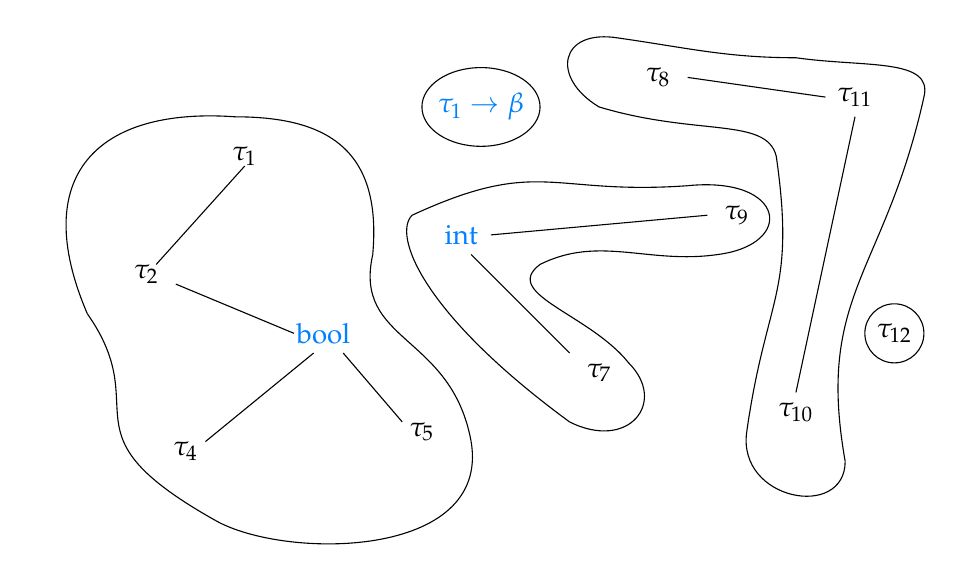
\begin{tikzpicture}[scale=0.5]

\node at (5,13.75) {$\tau_1$};
\node [color={rgb,255:red,0; green,128; blue,255}] at (7,9.25) {bool};
\node [color={rgb,255:red,0; green,128; blue,255}] at (11,15) {$\tau_1 \rightarrow \beta$};
\node [color={rgb,255:red,0; green,128; blue,255}] at (10.5,11.75) {int};
\node at (14,8.25) {$\tau_7$};
\node at (17.5,12.25) {$\tau_9$};
\node at (20.5,15.25) {$\tau_{11}$};
\node at (15.5,15.75) {$\tau_8$};
\node at (9.5,6.75) {$\tau_5$};
\node at (2.5,10.75) {$\tau_2$};
\node at (19,7.25) {$\tau_{10}$};
\node at (21.5,9.25) {$\tau_{12}$};
\node at (3.5,6.25) {$\tau_4$};
\draw (2.75,11) -- (5,13.5);
\draw (3.25,10.5) -- (6.25,9.25);
\draw (6.75,8.75) -- (4,6.5);
\draw (7.5,8.75) -- (9,7);
\draw (10.75,11.25) -- (13.25,8.75);
\draw (11.25,11.75) -- (16.75,12.25);
\draw (16.25,15.75) -- (19.75,15.25);
\draw (20.5,14.75) -- (19,7.75);
\draw (4.75,14.75) .. controls (7,14.75) and (8.5,14) .. (8.25,11.25);
\draw (8.25,11.25) .. controls (7.75,9) and (10.25,9.25) .. (10.75,6.5);
\draw (10.75,6.5) .. controls (11.25,3.5) and (6,3.5) .. (4.25,4.5);
\draw (4.25,4.5) .. controls (0.25,6.75) and (2.75,7.25) .. (1,9.75);
\draw (1,9.75) .. controls (-0.5,13.25) and (1.25,15) .. (4.75,14.75);
\draw  (11,15) ellipse (1.5cm and 1.0cm);
\draw (14,15) .. controls (16.5,14.25) and (18.25,14.75) .. (18.5,13.75);
\draw (18.5,13.75) .. controls (19,10.25) and (18.25,10.25) .. (17.75,6.75);
\draw (17.75,6.75) .. controls (17.5,5) and (20.25,4.5) .. (20.25,6);
\draw (20.25,6) .. controls (19.5,10.25) and (21.25,10.75) .. (22.25,15.25);
\draw (22.25,15.25) .. controls (22.5,16.25) and (20.75,16) .. (19,16.25);
\draw (19,16.25) .. controls (17.25,16.25) and (16.25,16.5) .. (14.5,16.75);
\draw (14.5,16.75) .. controls (13,17) and (12.75,15.75) .. (14,15);
\draw (9.25,12.25) .. controls (12.5,13.75) and (12.75,12.75) .. (16.25,13);
\draw (16.25,13) .. controls (18.75,13.25) and (19,11.5) .. (17,11.25);
\draw (17,11.25) .. controls (15.25,11) and (14,11.75) .. (12.5,11);
\draw (12.5,11) .. controls (11.5,10.25) and (13.75,9.75) .. (14.75,8.5);
\draw (14.75,8.5) .. controls (15.75,7.5) and (14.75,6.25) .. (13.25,7);
\draw (13.25,7) .. controls (9.5,9.75) and (8.75,11.75) .. (9.25,12.25);
\draw  (21.5,9.25) ellipse (0.75cm and 0.75cm);

\end{tikzpicture}
\end{center}


On voit que cet ensemble peut être représenté comme un graphe, où $\tau_i=\tau_j\iff\tau_i\longleftrightarrow \tau_j$. On en déduit que les composantes connexes sont les classes d'équivalences de la relation $(=)$ sur les types du contexte ! Une manière de résoudre un système d'équation est alors de fusionner les classes d'équivalences de deux types lorsqu'ils sont mis en égalité : cette tâche est facilement effectuée par la structure Union-Find.

Remarquons que si l'un des types dans une classe d'équivalence n'est pas une variable, alors ce type représente le type de la classe d'équivalence, et donc de toutes les expressions dont le type est dans la même classe.

Grâce à la structure Union-Find, on peut donc mettre à jour une partition du contexte $\Gamma$, tel que $\text{find}(\tau)$ est le représentant de cette classe. Attention, il faut imposer que $\text{find}(\tau)$ soit, dès que possible, un type qui n'est pas une variable, car le représentant sera la solution que l'on devra extraire des classes d'équivalences.

\begin{remark}
    L'algorithme que nous sommes en train de décrire est \textbf{l'algorithme d'inférence de Damas-Hindley-Milner}.
\end{remark}

\textbf{Quand résoudre les contraintes ?}

Notre algorithme va établir un système d'équations, mais quand va-t-il le résoudre ? Voici deux méthodes pour résoudre un système d'égalités dans le cadre de l'inférence de types. \begin{itemize}
    \item La première consiste à résoudre de fameux système après avoir généré tous les types et toutes les contraintes. C'est l'algorithme le plus formel, et s'appuie sur la méthode de substitution dans un système. Plus précisément, on exprime un type à partir d'autres à l'aide d'une équation, puis on enlève cette équation, et on remplace toutes les occurences de ce type par le nouveau. On recommence jusqu'à obtenir un système résolé.
    
    Cet algorithme s'appelle \textbf{l'algorithme W}.

    \item La deuxième méthode est plus << gloutonne >> : elle fusionne les classes d'équivalences dès qu'une nouvelle contrainte est générée, et vérifie que les représentants des classes sont bien compatibles (en imposant une nouvelle contrainte).
    
    Cet algorithme s'appelle \textbf{l'algorithme J}.
\end{itemize}

L'algorithme J est souvent plus simple à implémenter, et puisque nous travaillons avec la structure Union-Find, c'est celui-ci que nous allons utiliser.

\begin{remark}
    L'algorithme J s'exécute en $\mathcal{O}(n\alpha(n))$, où $n$ est le nombre total de types dans le contexte $\Gamma$. 

    ~

    \textbf{Rappel} : $\alpha$ est la fonction inverse d'Ackermann $(n\mapsto A(n, n))$, et grandit extrêmement lentement. En pratique, on ne dépassera jamais $\alpha(n) > 4$, ce qui rend la complexité quasi-linéaire en $n$.
    
    En effet, $A(4, 4)\approx 2^{2^{2^{2^{16}}}}$.
\end{remark}

\subsection{Algorithme J : une implémentation}

L'algorithme J est ici partiellement implémenté en OCaml.

\subsubsection{Préliminaires}

On va définir les structures que l'on manipule. Notamment, les expressions, les motifs, les types, etc. Pour chacune d'entre elles, on s'appuie sur la définition de la partie (4.1).

\begin{lstlisting}
type expr =
  | EVar of var
  | EFun of pat * expr
  | EApp of expr * expr
  | ELet of (pat * expr) * expr
  | ESeq of expr * expr
  | ETuple of expr array
  | EVariant of int * expr
  | EMatch of expr * (pat * expr) array
  | EBool of bool
  | EIf of expr * expr * expr
  | EAnd of expr * expr | EOr of expr * expr | ENot of expr
  | EInt of int
  | EAdd of expr * expr | ESub of expr * expr | EMul of expr * expr | EDiv of expr * expr
  | ENeg of expr
  | EEq of expr * expr | ENe of expr * expr
  | ELe of expr * expr | ELt of expr * expr
  | EGe of expr * expr | EGt of expr * expr
and pat = 
  | PVar of var
  | PTuple of pat array
  | PVariant of int * pat
  | PBool of bool
  | PInt of int
and var = int
and ty_id = int
and ty =
  | TVar of ty_id 
  | TTuple of ty_id array
  | TFun of ty_id * ty_id
  | TBool | TInt
\end{lstlisting}

\begin{remark}
    Je laisse intentionnellement un niveau d'indirection supplémentaires pour la structure des types, car quand j'utiliserai la structure Union-Find sur les types, je vais avoir besoin de faire références aux classes d'équivalences d'un type, et j'aurai donc besoin de son indice dans la structure U-F.
\end{remark}

\subsubsection{Contexte}

Rappelons-nous que le contexte doit être un tableau associatif, et un pointeur vers un contexte précédement pour prendre en compte le shadowing. Je propose la structure suivante :

\begin{lstlisting}
type ctx = {
  variables : (var, ty) Hashtbl.t ;
  prev : ctx option ;
}
\end{lstlisting}

Le premier contexte créé n'a pas de contexte parent, donc on l'initialise avec la fonction suivante :

\begin{lstlisting}
let ctx_init () = {
  variables = Hashtbl.create 0;
  prev = None;
}
\end{lstlisting}

La fonction suivante permet d'ajouter une nouvelle variable dans le contexte actuel par effet de bord. Cette action risque d'assombrir (shadow) une variable du même nom qui était déjà dans le contexte !

\begin{lstlisting}
let declare_variable ctx (var, ty) =
  Hashtbl.replace ctx.variables var ty
\end{lstlisting}

Enfin, la fonction suivante cherche le type d'une variable dans le contexte étant donné son identifiant. Il faut faire une recherche récursive :
\begin{itemize}
    \item Si la variable se trouve dans la portée actuelle, alors on renvoie son type.
    \item Sinon, on cherche dans la portée précédente.
    \item Si le contexte actuel est la racine, on émet une erreur : << Variable inconnue>>.
\end{itemize}

\begin{lstlisting}
exception Unknown_Variable of var
let rec find_variable ctx x =
  match Hashtbl.find_opt ctx.variables x with
  | Some ty -> ty
  | None -> match ctx.prev with
    | Some ctx' -> find_variable ctx' x
    | None -> raise (Unknown_Variable x)
\end{lstlisting}

Cela devrait être bon pour le contexte.

\newpage
\subsubsection{Union-Find}

Je ne vais pas détailler l'implémentation d'une structure Union-Find ici, mais voici sa signature :
\begin{lstlisting}
type 'a uf
uf_create: () -> 'a uf
uf_add: 'a uf -> 'a -> int
uf_find: 'a uf -> int -> int
uf_union: 'a uf -> int -> int -> unit
uf_get: 'a uf -> int -> 'a
\end{lstlisting}

Vous remarquerez peut-être qu'elle est un peu différente de ce qu'on a l'habitude d'utiliser. Oui, en effet. J'ai modifié la structure pour qu'elle stocke des valeurs de type \verb|'a|, ce qui me permettra de récupérer la valeur du représentant d'une classe d'équivalence.

\subsubsection{Unification des contraintes}

Pour résoudre le système, il faut que l'on fusionne deux classes d'équivalences si une égalité porte sur deux types inconnus. S'il les deux sont connus (i.e. ce ne sont pas des variables), on vérifie qu'ils sont bien égaux en regardant s'ils ont bien la même forme, et en ajoutant des contraintes supplémentaires sur leur types intérieurs. 

Cette étape s'appelle \textit{l'unification}.

En détail, l'algorithme se déroule de la manière suivante :
\begin{itemize}
    \item \textbf{Entrée} : deux types $\alpha'$ et $\beta'$ (représentés par un \verb|ty_id|, leur position dans la structure U-F).
    \item On récupère leur type réprésentant $\alpha$ et $\beta$, car ils sont égaux, et on veut raisonner sur les représentants des classes d'équivalence.
    \item \underline{Cas des variables : l'un d'entre eux est une variable}. Sans perte de généralité, on suppose que $\alpha$ et $x$.
    \begin{itemize}
        \item \textbf{On vérifie que $\alpha=x$ n'apparaît pas dans l'écriture de $\beta$ !!} On ne peut pas autoriser les types récursifs, donc si jamais c'est le cas, on émet une erreur : << Erreur de typage (type infini), $x\ne\beta$ >>.
        \item Si l'étape précédente a été vérifiée, alors on impose que $x=\beta$ en fusionnant les classes de $\alpha$ et $\beta$. En le faisant, \textbf{on s'assure que le nouveau représentant de cette classe soit $\beta$}, c'est-à-dire, après fusion, $\text{find}(\alpha)=\text{find}(\beta)=\beta$. On a déjà expliqué pourquoi ceci devait être le cas, c'est parce qu'on privilégie des types concrêts plutôt que des variables en tant que représentants.
    \end{itemize}

    \item \underline{$\alpha=\text{int}$ et $\beta=\text{int}$}. Il n'y a rien a vérifier d'autre, donc on retourne unit.
    \item \underline{$\alpha=\text{bool}$ et $\beta=\text{bool}$}. Idem.
    \item \underline{$\alpha=\tau_1\to\tau_2$ et $\beta=\mu_1\to\mu_2$}. On impose que $\tau_1 = \mu_1$ et que $\tau_2 = \mu_2$ en appelant récursivement l'algorithme d'unification sur l'entrée $(\tau_1, \mu_1)$ puis $(\tau_2, \mu_2)$.
    \item \underline{$\alpha=(\alpha_1, \dots, \alpha_n)$ et $\beta=(\beta_1, \dots, \beta_m)$}. D'une part, on vérifie manuellement que $m=n$, sinon erreur ! << Erreur de typage (taille de tuples incompatibles) >>.
    
    Ensuite, $\forall i\in\left\llbracket1, n\right\rrbracket$, on impose que $\alpha_i=\beta_i$ avec un appel récursif à l'unification.

    \item \underline{Autre cas} : les types ne peuvent pas être égaux, donc ont émet immédiatement une erreur. << Erreur de typage : $\alpha\ne\beta$ >>.
\end{itemize}

Tout d'abord, définissons une structure qui va contenir les informations utiles à l'inférence de type (le contexte et la structure U-F).

\begin{lstlisting}
type checker = {
  types: ty uf ;
  mutable context: ctx;
}
\end{lstlisting}

Ensuite, écrit la fonction qui vérifie si une variable $x$ apparaît dans l'écriture d'un type $\tau$.

On l'appelle \verb|occurs_in: checker -> ty_id -> ty_id -> bool|

\begin{lstlisting}
let rec occurs_in checker x tau =
  match uf_get checker.types tau with
  | TVar y -> x = y
  | TBool | TInt -> false
  | TFun (a, b) -> occurs_in checker x a || occurs_in checker x b
  | TTuple (tys) -> Array.exists (occurs_in checker x) tys
\end{lstlisting}

La fonction fait une disjonction de cas sur $\tau$, et si $\tau=y$, alors on vérifie que $x=y$, sinon, on effectue des appels récursivement en regardant si au moins l'un d'entre eux renvoie true.

La fonction \verb|unify: checker -> ty_id -> ty_id -> unit| s'écrit alors :
\begin{lstlisting}
exception Occurs_In_Fail of ty_id * ty_id
exception Type_Error of ty_id * ty_id
let rec unify checker a b =
  match (uf_get checker.types a, uf_get checker.types b) with
  | (TVar xa, _) -> if occurs_in checker xa b
      then raise (Occurs_In_Fail (a, b))
      else uf_union checker.types a b
  | (_, TVar xb) -> if occurs_in checker xb a
      then raise (Occurs_In_Fail (b, a))
      else uf_union checker.types b a
  | (TInt, TInt) -> ()
  | (TBool, TBool) -> ()
  | (TFun (t1, t2), TFun (u1, u2)) ->
      unify checker t1 u1;
      unify checker t2 u2;
  | (TTuple aa, TTuple bb) when Array.length aa = Array.length bb -> 
      let n = Array.length aa in
      for i = 0 to n - 1 do
        unify checker aa.(i) bb.(i)
      done
  | _ -> raise (Type_Error (a, b))
\end{lstlisting}

\subsubsection{Inférence}

Presque terminé, il ne reste plus qu'à générer des contraints en parcourant les expressions et les motifs dont on veut le type. On fait cela en générant des appels à \verb|unify|, qui s'occupe des classes d'équivalences.

\textbf{Comment générer les contraintes ?}

Il faut s'appuyer sur les règles d'inférences. Commençons par les motifs :

\begin{itemize}
    \item \textbf{Entrée} : un motif $p$. \textbf{Sortie} : son type $\tau$.
    \item Par disjonction de cas sur la forme de $p$, qui correspond à une règle d'inférence ({\scshape(T-Pat-)\dots}).
    \begin{itemize}
        \item \underline{$p=x$ une variable : règle ({\scshape{T-Pat-Ax}})}. On commence par créer un tout nouveau type $\alpha$ qui sera le type de $x$. On ajoute $(x:\alpha)$ au contexte $\Gamma$, puis on renvoie simplement $\alpha$.
        \item \underline{$p=\text{true}$ ou $p=\text{false}$ : règle ({\scshape{T-Pat-True}}) ou ({\scshape{T-Pat-False}})}. On renvoie directement le type $\text{bool}$.
        \item \underline{$p=n\in\mathbb{Z}$ : règle ({\scshape{T-Pat-Int}})}. On renvoie directement le type $\text{int}$.
        \item \underline{$p=(p_1, \dots, p_n)$ : règle ({\scshape{T-Pat-Tuple}}$\,_n$)}. On infère récursivement les motifs $p_1, \dots, p_n$, ce qui nous donne les types $\tau_1, \dots, \tau_n$, et on renvoie directement le type tuple formé de ces derniers : $\left(\tau_1, \dots, \tau_n\right)$.
        \item \underline{$p=\text{Var}_i~p'$ : règle ({\scshape{T-Pat}}-$\text{Var}_i$)}. On récupère les type $\tau_i$ associé au variant $\text{Var}_i$ de $\Sigma$. On procède récursivement en inférant le type $\tau'$ de $p'$, puis on vérifie $\tau_i=\tau'$ par unification. Enfin, on renvoie $\tau_i$.
    \end{itemize}
\end{itemize}

Je ne détaille pas comment j'obtiens le type d'un variant $\text{Var}_i$ (cela dépend en vérité de la structure de votre code), et je me donne une fonction magique qui le fait à ma place : \verb|get_variant : int -> ty_id|.

La fonction \verb|infer_pattern : checker -> pat -> ty_id| qui infére le type d'un motif peut être écrite comme ceci :

\begin{lstlisting}
let rec infer_pattern checker p =
    match p with
    | PVar x -> 
        let alpha = create_fresh_type checker in
        declare_variable checker.context (x, alpha);
        alpha
    | PBool _ -> create_type checker TBool
    | PInt _ -> create_type checker TInt
    | PTuple pp ->
        create_type checker
          (TTuple (Array.map (infer_pattern checker) pp))
    | PVariant (i, p') ->
        let tau_i = get_variant i in
        let tau' = infer_pattern checker p' in
        unify checker tau_i tau';
        tau_i    
\end{lstlisting}

Même raisonnement pour les expressions, sauf qu'il y a beaucoup plus de cas !

\begin{itemize}
    \item \textbf{Entrée} : une expression $e$. \textbf{Sortie} : son type $\tau$.
    \item Par disjonction de cas sur la forme de $e$, qui correspond à une règle d'inférence ({\scshape(T-)\dots}).
    \begin{itemize}
        \item \underline{$e=x$ une variable : règle ({\scshape{T-Ax}})}. On récupère le type de $x$ en fouillant dans le contexte, puis on le retourne. Si la variable n'existe pas, ceci émet une erreur.
        \item \underline{$e=\text{\lstinline|fun|}~p~\text{\lstinline|->|}~e'$ : règle ({\scshape{T-Abs}})}. Déjà, avant toute chose, on ouvre un nouveau contexte, pour empêcher les variables de la fonction d'en sortir. Dans ce contexte, on infère le motif $p:\tau_1$, \textit{et seulement après} on infère le corps de la fonction $e':\tau_2$. On ferme le contexte puis on renvoie le type $\tau_1\to\tau_2$.
        \item \underline{$e=f~e'$ : règle ({\scshape{T-App}})}. On commence par inférer le type de $f:\phi'$. Ensuite, on infère le type de l'argument $e':\alpha$, et on crée un nouveau type de retour $\beta$. On pose $\phi=\alpha\to\beta$, et on impose par unification que $\phi=\phi'$. Le type de retour de l'appel est $\beta$ d'après la règle d'inférence, donc c'est le type que l'on renvoie.
        \item \underline{$e=\text{\lstinline|let|}~p~\texttt{=}~e'~\text{\lstinline|in|}~e''$ : règle ({\scshape{T-Let}})}. Il faut que $e'$ puisse rentrer dans $p$ d'après la règle. On infère donc $p:\epsilon$ puis $e':\epsilon'$, et par unification, on impose $\epsilon=\epsilon'$. Il ne reste qu'à renvoyer le type de $e'':\tau$, que l'on infère récursivement.
        \item \underline{$e=e'~\texttt{;}~e''$ : règle ({\scshape{T-Seq}})}. On impose par unification que le type inféré de $e:\tau'$ soit $\tau'=()$, puis on renvoie l'inférence du type de $e''$ immédiatement.
        \item \underline{$e=\text{true}$ ou $p=\text{false}$ : règle ({\scshape{T-True}}) ou ({\scshape{T-False}})}. Idem que pour les motifs true ou false.
        \item \underline{$e=\text{\lstinline|if|}~g~\text{\lstinline|then|}~a~\text{\lstinline|else|}~b$ : règle ({\scshape{T-If}})}. On impose par unification que le type inféré de $g:\gamma$ soit $\gamma=\text{bool}$. Ensuite, on infère les types des deux valeurs possibles, $a:\tau_a$ et $b:\tau_b$, puis on impose par unification que $\tau_a=\tau_b=\tau$. On renvoie $\tau$.
        \item \underline{$e=n\in\mathbb{Z}$ : règle ({\scshape{T-Int}})}. Idem que pour le motif entier.
        \item \underline{$e=(p_1, \dots, p_n)$ : règle ({\scshape{T-Tuple}}$\,_n$)}. Idem que pour le motif $n$-uplet.
        \item \underline{$e=\text{Var}_i~p'$ : règle ({\scshape{T-}}-$\text{Var}_i$)}. Idem que pour le motif du variant $\text{Var}_i$.
        \item \underline{$e=\text{\lstinline|match|}~s~\text{\lstinline|with|}~\texttt{|}~p_1~\texttt{->}~e_1~\texttt{|}~\dots~\texttt{|}~p_n~\texttt{->}~e_n$ : règle ({\scshape{T-Match}})}. Inférons d'abord le type de $s:\sigma$, puis créons un nouveau type frais $\tau$. Pour chaque cas $i\in\left\llbracket1, n\right\rrbracket$, on infère les types $e_i:\tau_i$ et $p_i:\sigma_i$. D'après la règle, tous les motifs doivent être du type $\sigma$, donc on impose par unification que $\sigma_i=\sigma$. De même, toutes les valeurs de retour doivent être $\tau$, donc par unification on impose $\tau_i=\tau$. Il ne reste plus qu'à renvoyer $\tau$.
        \item \underline{Dans le cas où $e$ est une opération sur les booléens, les entiers, ou une opération de comparison}
        
        On applique la règle respective ({\scshape{T-$\diamond$}}). Il faut que les types inférés de ou des arguments soient égaux (imposé par unification). Si l'opération est sur les entiers, on impose en plus que le ou les arguments soient entiers par unification. Idem pour les booléens. On renvoie le type associé au résultat de l'opération : c'est un entier si c'est une opération arithmétiques, un booléen si c'est une opération booléenne, et sinon un booléen si c'est un test.
    \end{itemize}
\end{itemize}

Wouah, nous y sommes ! La fonction codée en OCaml, \verb|infer : checker -> expr -> ty_id|, est :
\begin{lstlisting}
let rec infer checker e = 
  match e with
  | EVar x -> find_variable checker.context x
  | EFun (p, e') ->
      open_scope checker;
      let arg = infer_pattern checker p in
      let ret = infer checker e' in
      close_scope checker;
      create_type checker (TFun (arg, ret))
  | EApp (f, e') ->
      let phi' = infer checker f in
      let arg = infer checker e' in
      let ret = create_fresh_type checker in
      let phi = create_type checker (TFun (arg, ret)) in
      unify checker phi phi';
      ret
  | ELet ((p, e'), e'') ->
      let eps = infer_pattern checker p in
      let eps' = infer checker e' in
      unify checker eps eps';
      infer checker e''
  | ESeq (e', e'') -> 
      let unit = create_type checker (TTuple [||]) in
      unify checker unit (infer checker e');
      infer checker e''
  | EBool _ -> create_type checker TBool
  | EIf (g, a, b) -> 
      let bool = create_type checker TBool in
      unify checker bool (infer checker g);
      let tau_a = infer checker a in
      let tau_b = infer checker b in
      unify checker tau_a tau_b;
      tau_a
  | EInt _ -> create_type checker TInt
  | ETuple ee ->
      create_type checker
        (TTuple (Array.map (infer checker) ee))
  | EVariant (i, p') ->
      let tau_i = get_variant i in
      let tau' = infer checker p' in
      unify checker tau_i tau';
      tau_i
  | EMatch (s, cases) -> 
      let sigma = infer checker s in
      let tau = create_fresh_type checker in
      Array.iter (fun (p, e) -> 
        let sigma' = infer_pattern checker p in
        let tau' = infer checker e in
        unify checker sigma sigma';
        unify checker tau tau';
      ) cases; tau
  | EAdd (a, b) | ESub (a, b) | EMul (a, b) | EDiv (a, b) ->
      let int = create_type checker TInt in
      unify checker int (infer checker a);
      unify checker int (infer checker b);
      int
  | ENeg e' ->
      let int = create_type checker TInt in
      unify checker int (infer checker e');
      int
  | EAnd (a, b) | EOr (a, b) ->
      let bool = create_type checker TBool in
      unify checker bool (infer checker a);
      unify checker bool (infer checker b);
      bool
  | ENot e' ->
      let bool = create_type checker TBool in
      unify checker bool (infer checker e');
      bool
  | EEq (a, b) | ENe (a, b)
  | ELe (a, b) | ELt (a, b)
  | EGe (a, b) | EGt (a, b) ->
      let tau = create_fresh_type checker in
      unify checker tau (infer checker a);
      unify checker tau (infer checker b);
      create_type checker TBool
\end{lstlisting}

Bravo !

\section{Extensions et autres systèmes de typage}
\subsection{Polymorphisme, types quantifiés}
\subsection{Sous-typage}
\subsection{Contraintes sémantiques}

\newpage
\section*{Bibliographie}
\begin{itemize}
    \item {\scshape{Benjamin C. Pierce}}, \href{https://www.cis.upenn.edu/~bcpierce/tapl/}{\textbf{Types and Programming Languages}}
    \item {\scshape{Yves Bertot}}, \href{https://www-sop.inria.fr/members/Yves.Bertot/courses/lambda-pur.pdf}{\textbf{Introduction au lambda-calcul pur}} -- issu d'un ADS de l'X.
\end{itemize}

\end{document}